\chapter{作业}
\section{第一周作业}
\begin{homework}{3}
    汽车制造商的生产记录表明了每个班的产品数量（每个班的最大产量是 720 辆汽车）。
    \begin{center}
        \begin{tabular}{ccccccccccccc}
            668 & 711 & 625 & 701 & 688 & 667 & 694 & 630 & 547 & 703 & 688 & 697 & 703 \\
            656 & 677 & 700 & 702 & 688 & 691 & 664 & 688 & 679 & 708 & 699 & 667 & 703 \\
        \end{tabular}
    \end{center}
    \begin{enumerate}
        \item 画出茎叶图。
        \item 计算样本均值和样本中位数。
        \item 均值和中位数间的关系关于数据的形状说明了什么？
    \end{enumerate}
\end{homework}
\begin{solution}



(1) 使用 R 语言的 \texttt{stem()} 函数处理该组生产记录数据。为了使茎叶图的结构更加紧凑并消除不必要的空行，我们将 \texttt{scale} 参数调整为 $0.5$。得到结果如下：

\begin{lstlisting}[language=R]
> data <- c(668, 711, 625, 701, 688, 667, 694, 630, 547, 703, 688, 697, 703,
+           656, 677, 700, 702, 688, 691, 664, 688, 679, 708, 699, 667, 703)
> stem(data, scale = 0.5)

  The decimal point is 1 digit(s) to the right of the |

  54 | 7
  56 | 
  58 | 
  60 | 
  62 | 50
  64 | 6
  66 | 4777879
  68 | 88881479
  70 | 01233381
\end{lstlisting}

(2) 利用 R 语言中的 \texttt{mean()} 和 \texttt{median()} 函数计算样本统计量：
\begin{itemize}
    \item \textbf{样本均值}：$\bar{x} \approx 678.6154$
    \item \textbf{样本中位数}：$M = 688$
\end{itemize}

(3) 根据计算结果可知，$\text{均值} (678.6154) < \text{中位数} (688)$。
在统计学中，当均值小于中位数时，通常说明数据分布呈现\textbf{左偏（负偏态）}。这反映出生产记录中存在极少数产量显著较低的班次（如 $547$），这些“长尾”数据拉低了整体的平均水平，使得分布曲线向左延伸。

\end{solution}
\begin{homework}{4}
    在一项血清胆固醇含量 (mg/L) 的研究中，记录了 20 个成年患者的胆固醇含量：
    \begin{center}
        \begin{tabular}{cccccccccc}
            133 & 137 & 148 & 149 & 152 & 167 & 174 & 179 & 189 & 192 \\
            201 & 209 & 210 & 211 & 218 & 238 & 245 & 248 & 253 & 257 \\
        \end{tabular}
    \end{center}
    试求 (1) 样本均值和样本中位数；(2) 极差、四分位数间距和样本方差。
\end{homework}
\begin{solution}
(1) 利用 R 语言中的 \texttt{mean()} 和 \texttt{median()} 函数计算样本统计量：
\begin{itemize}
    \item \textbf{样本均值}：$\bar{x} = 195.5$
    \item \textbf{样本中位数}：$M = 196.5$
\end{itemize}

(2) 利用 R 语言计算该组数据的离散程度指标：
\begin{itemize}
    \item \textbf{极差 (Range)}：$R = \max(x) - \min(x) = 257 - 133 = 124$。
    \item \textbf{四分位数间距 (IQR)}：通过 \texttt{IQR()} 函数计算得到 $\text{IQR} = Q_3 - Q_1 = 59.75$。
    \item \textbf{样本方差 (Sample Variance)}：使用 \texttt{var()} 函数计算（采用 $n-1$ 修正）：
    $$s^2 = \frac{1}{n-1} \sum_{i=1}^{n} (x_i - \bar{x})^2 \approx 1605.842$$
\end{itemize}
\end{solution}
\begin{homework}{5}
    用上题中的观测值画出箱线图，并由此说明总体分布的形状。
\end{homework}
\begin{center}
    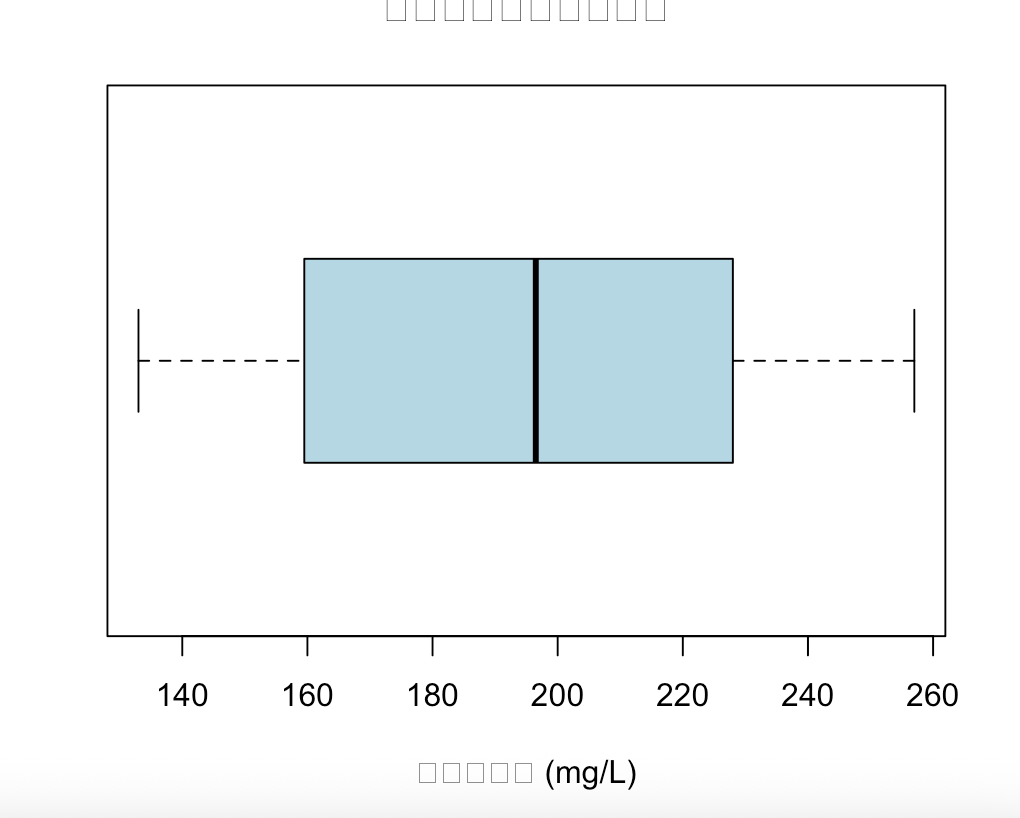
\includegraphics[width=0.5\linewidth]{3.9.png}
    
    \label{fig:placeholder}

 
\end{center}
\begin{solution}使用 R 语言绘制血清胆固醇含量的箱线图（见上图），并结合图形特征对总体分布形状进行分析：\begin{itemize}\item \textbf{对称性分析}：从图中可以看出，中位数（箱体中的黑实线）位置稍稍偏向箱体的右侧（靠近上四分位数 $Q_3$），且左侧的须线（whisker）相对于右侧须线略长。\item \textbf{偏态说明}：结合上题计算结果，均值 ($\bar{x} = 195.5$) 小于中位数 ($M = 196.5$)。箱线图呈现出左侧间距（最小值到中位数）略大于右侧间距（最大值到中位数）的特征，这表明总体分布呈现轻微的\textbf{左偏（负偏态）}分布。\item \textbf{离群值判断}：在箱线图的上下须线之外未发现孤立的点，说明在该样本数据中不存在明显的异常值（离群点）。\end{itemize}\end{solution}
\subsection*{page44}

\begin{homework}[3]
设 $X_1, X_2, \cdots, X_n$ i.i.d., $X_1 \sim N(\mu,\sigma^2)$，其中 $\mu$ 是已知数，而 $\sigma^2$ 是未知的，指出下列各量哪些是统计量，哪些不是统计量，并说明理由：
\[
\sum_{i=1}^n X_i,\qquad
X_1+2\mu,\qquad
\max_{1\le i\le n}\{X_i\},\qquad
\sum_{i=1}^n \frac{(X_i-\mu)^2}{\sigma^2},\qquad
\sum_{i=1}^n (X_i-\mu)^2.
\]
\end{homework}
\begin{dxtips}
统计量只能由样本 $X_1,\dots,X_n$ 和已知常数构成
\end{dxtips}
\begin{solution}
    是，是，是，不是，是
\end{solution}
\begin{note}
统计量就是：拿到一组真实样本数据后，对这些数据做具体运算得到的结果。

例如测得
\[
x_1,x_2,\dots,x_n,
\]
则相加、取平均、取最大值、排序、求平方和等得到的量，通常都是统计量。
\end{note}
\begin{homework}[4]
某机床加工出的零件的直径服从正态分布 $N(\mu,\sigma^2)$，$\mu,\sigma^2$ 未知。为对 $\mu,\sigma^2$ 作出估计，随机选取加工出来的 $n$ 个零件进行测量，得到 $n$ 个数据
\[
x_1,x_2,\cdots,x_n.
\]
试写出该问题的统计模型（即参数空间和样本分布族）。
\end{homework}
\begin{solution}
设
\[
X_1,X_2,\cdots,X_n
\]
为随机选取的 $n$ 个零件直径，由题意可知
\[
X_1,X_2,\cdots,X_n \overset{\text{i.i.d.}}{\sim} N(\mu,\sigma^2),
\]
其中参数 $\mu,\sigma^2$ 均未知。

因此，该问题的统计模型可写为：
\begin{itemize}
    \item 参数空间为
    \[
    \Theta=\{(\mu,\sigma^2):\mu\in\mathbb{R},\ \sigma^2>0\}.
    \]

    \item 样本分布族为：样本 $(X_1,X_2,\cdots,X_n)$ 的联合概率密度为
    \[
    f(x_1,x_2,\cdots,x_n;\mu,\sigma^2)
    =\prod_{i=1}^n \frac{1}{\sqrt{2\pi}\sigma}
    \exp\!\left[-\frac{(x_i-\mu)^2}{2\sigma^2}\right],
    \qquad (\mu,\sigma^2)\in\Theta.
    \]
\end{itemize}

故该问题的统计模型就是由参数空间
\[
\Theta=\{(\mu,\sigma^2):\mu\in\mathbb{R},\ \sigma^2>0\}
\]
和样本分布族
\[
\left\{
P_{\mu,\sigma^2}:(X_1,\dots,X_n)\overset{\text{i.i.d.}}{\sim}N(\mu,\sigma^2),
\ (\mu,\sigma^2)\in\Theta
\right\}
\]
所组成的统计模型。
\end{solution}
\begin{homework}[6]
（柯西分布）设 $X_1,X_2,\cdots,X_n$ i.i.d.，$X_1$ 服从柯西分布，概率密度为
\[
f(x,\sigma)=\frac{1}{\pi\sigma}\frac{1}{1+(x/\sigma)^2},\qquad -\infty<x<\infty,
\]
求
\[
\overline{X}=\frac{1}{n}\sum_{i=1}^n X_i
\]
的抽样分布。
\end{homework}
\begin{solution}
设每个样本的特征函数为
\[
\varphi_X(t)=E(e^{itX}).
\]
由柯西分布的已知结论，
\[
X_i\sim \mathrm{Cauchy}(0,\sigma)
\quad\Longrightarrow\quad
\varphi_{X_i}(t)=e^{-\sigma|t|}.
\]

由于 $X_1,X_2,\cdots,X_n$ 相互独立，故
\[
\varphi_{\overline X}(t)
=
E\!\left(e^{it\overline X}\right)
=
E\!\left(e^{it\frac{1}{n}\sum_{i=1}^n X_i}\right)
=
\prod_{i=1}^n E\!\left(e^{i(t/n)X_i}\right).
\]
于是
\[
\varphi_{\overline X}(t)
=
\prod_{i=1}^n \varphi_{X_i}\!\left(\frac tn\right)
=
\left(e^{-\sigma|t|/n}\right)^n
=
e^{-\sigma|t|}.
\]
\begin{dxtips}
\text{independent and identically distributed}相互独立而且同分布所以第二行能写成n次方，第一行只是把加号从指数取下来变成了乘法
\end{dxtips}
这正是参数为 $\sigma$ 的柯西分布的特征函数，因此
\[
\overline X \sim \mathrm{Cauchy}(0,\sigma).
\]

故 $\overline X$ 的抽样分布仍为柯西分布，其概率密度为
\[
f_{\overline X}(x)
=
\frac{1}{\pi\sigma}\frac{1}{1+(x/\sigma)^2},
\qquad -\infty<x<\infty.
\]
\end{solution}
\begin{dxtips}
    题目要求样本均值
\[
\overline{X}=\frac{1}{n}\sum_{i=1}^{n}X_i
\]
的抽样分布，即确定 \(\overline{X}\) 服从什么分布并求出其密度函数。

由于直接由密度求 \(\overline{X}\) 的分布需要进行多重卷积，计算较为繁琐，因此转而先求 \(\overline{X}\) 的特征函数，再由特征函数来确定其分布。

求得 \(\overline{X}\) 的特征函数后，将其与已知分布的特征函数进行比较，识别出 \(\overline{X}\) 所服从的分布，进而写出其密度函数，从而得到所求的抽样分布。
\end{dxtips}
\subsection*{page45}

\begin{homework}[1]
证明 $(2.2.3)$ 式。
\end{homework}
\begin{solution}
设
\[
S(p)=\sum_{k=r}^{n} C_n^k p^k(1-p)^{n-k}.
\]
对 \(p\) 求导，并利用\textcolor{red}{重点等式}
\[
kC_n^k=nC_{n-1}^{k-1},\qquad (n-k)C_n^k=nC_{n-1}^k,
\]
得
\begin{align*}
S'(p)
&=\sum_{k=r}^{n} C_n^k \Bigl[kp^{k-1}(1-p)^{n-k}-(n-k)p^k(1-p)^{n-k-1}\Bigr] \\
&=n\sum_{k=r}^{n} C_{n-1}^{k-1} p^{k-1}(1-p)^{n-k}
-n\sum_{k=r}^{n} C_{n-1}^k p^k(1-p)^{n-k-1}.
\end{align*}
在第一项中令 \(j=k-1\)，则
\[
S'(p)
=n\sum_{j=r-1}^{n-1} C_{n-1}^j p^j(1-p)^{n-1-j}
-n\sum_{k=r}^{n-1} C_{n-1}^k p^k(1-p)^{n-1-k}
=nC_{n-1}^{r-1}p^{r-1}(1-p)^{n-r}.
\]
再由
\[
nC_{n-1}^{r-1}=rC_n^r
\]
可得
\[
S'(p)=rC_n^r p^{r-1}(1-p)^{n-r}.
\]
两边从 \(0\) 到 \(p\) 积分，并注意 \(S(0)=0\)，于是
\[
S(p)=rC_n^r\int_0^p t^{r-1}(1-t)^{n-r}\,dt.
\]
故
\[
\sum_{k=r}^{n} C_n^k p^k(1-p)^{n-k}
=
rC_n^r\int_0^p t^{r-1}(1-t)^{n-r}\,dt.
\]
\end{solution}
\begin{dxtips}
    这个证明一边有积分一边没积分就应该想导是对左边求导然后再从0到p积分
\end{dxtips}
\begin{homework}[2]
（几何分布）设总体 $X$ 服从几何分布
\[
P\{X=k\}=p(1-p)^{k-1},\qquad k=1,2,\cdots,
\]
$X_1,X_2,\cdots,X_n$ 是抽自 $X$ 的简单随机样本，求 $X_{(1)},X_{(n)}$ 的分布。
\end{homework}
\begin{solution}
设
\[
q=1-p,\qquad X_{(1)}=\min\{X_1,\dots,X_n\},\qquad X_{(n)}=\max\{X_1,\dots,X_n\}.
\]
由于总体服从几何分布，
\[
P(X=k)=pq^{k-1},\qquad k=1,2,\dots,
\]
故对任意 \(m=1,2,\dots\)，有
\[
P(X>m)=q^m,\qquad P(X\le m)=1-q^m.
\]

\textbf{1. 求 \(X_{(1)}\) 的分布}

由次序统计量的分布公式，
\[
P\bigl(X_{(1)}>m\bigr)=P(X_1>m,\dots,X_n>m)=\bigl(P(X>m)\bigr)^n=q^{mn},
\]
因此
\[
P\bigl(X_{(1)}\le m\bigr)=1-q^{mn}.
\]
从而
\[
P\bigl(X_{(1)}=m\bigr)
=
P\bigl(X_{(1)}>m-1\bigr)-P\bigl(X_{(1)}>m\bigr)
=
q^{(m-1)n}-q^{mn}
=
(1-q^n)q^{(m-1)n},
\]
其中 \(m=1,2,\dots\).
\begin{dxtips}
    分布函数所有人都有就是小于等于m的概率。分布列只有离散型有就是P（X=x），概率密度函数只有连续型有因为只有连续型的分布函数才能求导。最大最小值求的时候不是只有他大于m的概率而是他能要求其他元素也满足这个条件。
\end{dxtips}
\textbf{2. 求 \(X_{(n)}\) 的分布}

由次序统计量的分布公式，
\[
P\bigl(X_{(n)}\le m\bigr)=P(X_1\le m,\dots,X_n\le m)=\bigl(P(X\le m)\bigr)^n=(1-q^m)^n,
\]
因此
\[
P\bigl(X_{(n)}=m\bigr)
=
P\bigl(X_{(n)}\le m\bigr)-P\bigl(X_{(n)}\le m-1\bigr)
=
(1-q^m)^n-(1-q^{m-1})^n,
\]
其中 \(m=1,2,\dots\).
\end{solution}
\begin{homework}[3]
（均匀分布）设 $X_1,X_2,\cdots,X_n$ i.i.d., $X_1\sim U\!\left[\theta-\frac12,\theta+\frac12\right]$，试分别求出 $X_{(1)}$ 和 $X_{(n)}$ 的概率密度。
\end{homework}
\section{第二次作业}

\subsection{45,3,4,6}
\begin{homework}{3}
设 $X_1, X_2, \cdots, X_n$ i.i.d., $X_1 \sim U\left[\theta - \frac{1}{2}, \theta + \frac{1}{2}\right]$, 试分别求出 $X_{(1)}$ 和 $X_{(n)}$ 的概率密度。
\end{homework}
\begin{solution}
    已知总体 $X \sim U[\theta - \frac{1}{2}, \theta + \frac{1}{2}]$，其概率密度函数 $f(x)$ 和分布函数 $F(x)$ 分别为：
    \[ 
    f(x) = \begin{cases} 1, & \theta - \frac{1}{2} \le x \le \theta + \frac{1}{2} \\ 0, & \text{其他} \end{cases} 
    \]
    \[ 
    F(x) = \begin{cases} 0, & x < \theta - \frac{1}{2} \\ x - \theta + \frac{1}{2}, & \theta - \frac{1}{2} \le x \le \theta + \frac{1}{2} \\ 1, & x > \theta + \frac{1}{2} \end{cases} 
    \]

    \paragraph{1. 求 $X_{(n)}$ 的概率密度}
    根据次序统计量的概率密度公式，$X_{(n)}$ 的密度函数为：
    \[ f_{X_{(n)}}(x) = n[F(x)]^{n-1}f(x) \]
    代入得：
    \[ 
    f_{X_{(n)}}(x) = \begin{cases} n(x - \theta + \frac{1}{2})^{n-1}, & \theta - \frac{1}{2} \le x \le \theta + \frac{1}{2} \\ 0, & \text{其他} \end{cases} 
    \]

    \paragraph{2. 求 $X_{(1)}$ 的概率密度}
    根据次序统计量的概率密度公式，$X_{(1)}$ 的密度函数为：
    \[ f_{X_{(1)}}(x) = n[1 - F(x)]^{n-1}f(x) \]
    由于当 $\theta - \frac{1}{2} \le x \le \theta + \frac{1}{2}$ 时：
    \[ 1 - F(x) = 1 - (x - \theta + \frac{1}{2}) = \theta + \frac{1}{2} - x \]
    代入得：
    \[ 
    f_{X_{(1)}}(x) = \begin{cases} n(\theta + \frac{1}{2} - x)^{n-1}, & \theta - \frac{1}{2} \le x \le \theta + \frac{1}{2} \\ 0, & \text{其他} \end{cases} 
    \]
\end{solution}
\begin{homework}{4}
设 $X_1, X_2, \cdots, X_n$ i.i.d., $X_1 \sim F(x)$, $F(x)$ 有概率密度 $f(x)$, 求：
\begin{enumerate}
    \item $X_{(1)}$ 和 $X_{(n)}$ 的联合分布函数及联合概率密度；
    \item $R = X_{(n)} - X_{(1)}$ 的分布函数及概率密度。
\end{enumerate}
\end{homework}
\begin{dxtips}
    大写是虚指小写是真实的数
\end{dxtips}
\begin{solution}
设
\[
U=X_{(1)}=\min\{X_1,\dots,X_n\},\qquad V=X_{(n)}=\max\{X_1,\dots,X_n\}.
\]

先求联合分布函数
\[
F_{U,V}(x,y)=P(U\le x,\ V\le y).
\]

由顺序统计量的定义分情况讨论：

\begin{itemize}
    \item 当 $x>y$ 时，由于 $U\le V$ 恒成立，
    \[
    \{U\le x,\ V\le y\}=\{V\le y\},
    \]
    故
    \[
    F_{U,V}(x,y)=P(V\le y)=P(X_1\le y,\dots,X_n\le y)=[F(y)]^n.
    \]

    \item 当 $x\le y$ 时，
    \[
    F_{U,V}(x,y)=P(V\le y)-P(U>x,\ V\le y).
    \]
    其中
    \[
    P(V\le y)=[F(y)]^n,
    \]
    而事件 $\{U>x,\ V\le y\}$ 表示所有样本都落在区间 $(x,y]$ 内，因此
    \[
    P(U>x,\ V\le y)=\bigl(F(y)-F(x)\bigr)^n.
    \]
    \begin{dxtips}
        这里本质决定的是X的积分区域
    \end{dxtips}
    从而
    \[
    F_{U,V}(x,y)=[F(y)]^n-\bigl(F(y)-F(x)\bigr)^n.
    \]
\end{itemize}

综上，
\[
F_{X_{(1)},X_{(n)}}(x,y)=
\begin{cases}
[F(y)]^n-\bigl(F(y)-F(x)\bigr)^n, & x\le y,\\[0.5em]
[F(y)]^n, & x>y.
\end{cases}
\]

下面求联合概率密度。对区域 $x<y$，有
\[
f_{X_{(1)},X_{(n)}}(x,y)
=\frac{\partial^2}{\partial x\,\partial y}F_{X_{(1)},X_{(n)}}(x,y).
\]
由
\[
F_{X_{(1)},X_{(n)}}(x,y)=[F(y)]^n-\bigl(F(y)-F(x)\bigr)^n
\]
求偏导得
\[
f_{X_{(1)},X_{(n)}}(x,y)
=n(n-1)\bigl(F(y)-F(x)\bigr)^{n-2}f(x)f(y),\qquad x<y.
\]

因此联合概率密度为
\[
f_{X_{(1)},X_{(n)}}(x,y)=
\begin{cases}
n(n-1)\bigl(F(y)-F(x)\bigr)^{n-2}f(x)f(y), & x<y,\\[0.5em]
0, & x\ge y.
\end{cases}
\]
\end{solution}
\begin{dxtips}[U和V不是独立的最大值的选取限制最小值]
    也就是说，知道“所有样本都不超过 $y$”以后，最小值落到 $x$ 左边的概率已经变了。

\medskip

更直观地说，事件 $V\le y$ 会限制样本全都待在 $(-\infty,y]$ 里。在这个前提下，再看 $U\le x$，它就不是原来那个无条件概率了。
\end{dxtips}
\begin{solution}
设
\[
U=X_{(1)},\qquad V=X_{(n)},\qquad R=V-U,\qquad T=U.
\]
则
\begin{dxtips}
    这个T的选取是任意可以和R凑出来v就行当你要把一个随机变量组换成另一个随机变量组，并且要从“旧变量的密度”推出“新变量的密度”时，就该想到雅可比行列式，因为边缘密度总是好求的
\end{dxtips}
\[
U=T,\qquad V=T+R.
\]
故雅可比行列式为
\[
J=\left|\frac{\partial(u,v)}{\partial(t,r)}\right|
=
\begin{vmatrix}
1 & 0\\
1 & 1
\end{vmatrix}
=1.
\]
于是
\[
f_{T,R}(t,r)=f_{U,V}(t,t+r),\qquad r>0.
\]
由第一问的结果，
\[
f_{U,V}(u,v)=n(n-1)\bigl(F(v)-F(u)\bigr)^{n-2}f(u)f(v),\qquad u<v.
\]
因此
\[
f_R(r)=\int_{-\infty}^{\infty} f_{T,R}(t,r)\,dt
=\int_{-\infty}^{\infty} f_{U,V}(t,t+r)\,dt
\]
\[
= n(n-1)\int_{-\infty}^{\infty}
\bigl(F(t+r)-F(t)\bigr)^{n-2}f(t)f(t+r)\,dt,\qquad r>0.
\]
并且
\[
f_R(r)=0,\qquad r\le 0.
\]
\end{solution}
\begin{homework}[5]
从某总体抽取一个容量为 $5$ 的样本：
\[
-2.8,\ -1,\ 1.5,\ 2.1,\ 3.4.
\]
写出该样本的经验分布函数并画出它的图形。
\end{homework}
\begin{solution}
将样本按从小到大排列为
\[
x_{(1)}=-2.8,\quad x_{(2)}=-1,\quad x_{(3)}=1.5,\quad x_{(4)}=2.1,\quad x_{(5)}=3.4.
\]

经验分布函数定义为
\[
F_n(x)=\frac{1}{n}\sum_{i=1}^n I\{x_i\le x\}.
\]
这里 \(n=5\)，所以
\[
F_5(x)=
\begin{cases}
0, & x<-2.8,\\[4pt]
\dfrac15, & -2.8\le x<-1,\\[6pt]
\dfrac25, & -1\le x<1.5,\\[6pt]
\dfrac35, & 1.5\le x<2.1,\\[6pt]
\dfrac45, & 2.1\le x<3.4,\\[6pt]
1, & x\ge 3.4.
\end{cases}
\]

其图形是一个右连续的阶梯函数，在
\[
x=-2.8,\ -1,\ 1.5,\ 2.1,\ 3.4
\]
这五个点处分别向上跳跃 \(\frac15\)。

可用下列 TikZ 代码作图：
\[
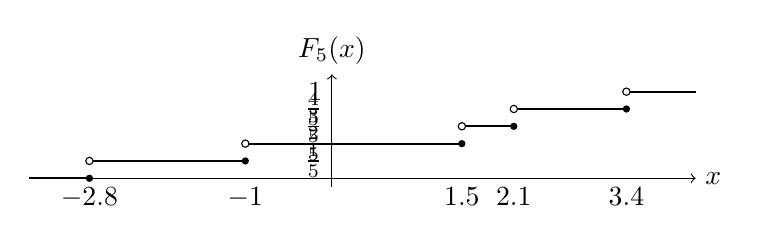
\begin{tikzpicture}[scale=1.1]
\draw[->] (-3.5,0) -- (4.2,0) node[right] {\(x\)};
\draw[->] (0,-0.1) -- (0,1.2) node[above] {\(F_5(x)\)};

\draw[thick] (-3.5,0) -- (-2.8,0);
\draw[thick] (-2.8,0.2) -- (-1,0.2);
\draw[thick] (-1,0.4) -- (1.5,0.4);
\draw[thick] (1.5,0.6) -- (2.1,0.6);
\draw[thick] (2.1,0.8) -- (3.4,0.8);
\draw[thick] (3.4,1) -- (4.2,1);

\fill (-2.8,0) circle (1.2pt);
\fill (-1,0.2) circle (1.2pt);
\fill (1.5,0.4) circle (1.2pt);
\fill (2.1,0.6) circle (1.2pt);
\fill (3.4,0.8) circle (1.2pt);

\draw[fill=white] (-2.8,0.2) circle (1.2pt);
\draw[fill=white] (-1,0.4) circle (1.2pt);
\draw[fill=white] (1.5,0.6) circle (1.2pt);
\draw[fill=white] (2.1,0.8) circle (1.2pt);
\draw[fill=white] (3.4,1) circle (1.2pt);

\node[below] at (-2.8,0) {\(-2.8\)};
\node[below] at (-1,0) {\(-1\)};
\node[below] at (1.5,0) {\(1.5\)};
\node[below] at (2.1,0) {\(2.1\)};
\node[below] at (3.4,0) {\(3.4\)};

\node[left] at (0,0.2) {\(\frac15\)};
\node[left] at (0,0.4) {\(\frac25\)};
\node[left] at (0,0.6) {\(\frac35\)};
\node[left] at (0,0.8) {\(\frac45\)};
\node[left] at (0,1) {\(1\)};
\end{tikzpicture}
\]
\end{solution}
\begin{dxtips}
    经验分布函数就是：看样本里有多少比例不超过 x。图像的纵轴就是累积比例，横轴就是具体的节点。也就是F5（x）图像
\end{dxtips}
\begin{homework}{6}
证明：正态分布 $N(\mu, \sigma^2)$ 的上 $\alpha$ ($0 < \alpha < 1$) 分位数 $z_\alpha$ 与标准正态分布的上 $\alpha$ 分位数 $u_\alpha$ 之间有以下关系：
$$z_\alpha = \mu + \sigma u_\alpha$$
\end{homework}
\begin{proof}
设
\[
X\sim N(\mu,\sigma^2),\qquad Y=\frac{X-\mu}{\sigma}.
\]
则
\[
Y\sim N(0,1).
\]

由上 \(\alpha\) 分位数的定义，\(z_\alpha\) 满足
\[
P(X>z_\alpha)=\alpha,
\]
而标准正态分布的上 \(\alpha\) 分位数 \(u_\alpha\) 满足
\[
P(Y>u_\alpha)=\alpha.
\]

另一方面，
\[
P(X>z_\alpha)
=
P\left(\frac{X-\mu}{\sigma}>\frac{z_\alpha-\mu}{\sigma}\right)
=
P\left(Y>\frac{z_\alpha-\mu}{\sigma}\right).
\]
因此
\[
P\left(Y>\frac{z_\alpha-\mu}{\sigma}\right)=\alpha.
\]

又因为 \(u_\alpha\) 是标准正态分布的上 \(\alpha\) 分位数，即满足
\[
P(Y>u_\alpha)=\alpha,
\]
故必有
\[
\frac{z_\alpha-\mu}{\sigma}=u_\alpha.
\]
于是
\[
z_\alpha=\mu+\sigma u_\alpha.
\]

故证。
\end{proof}
\subsection{46,1,2,3}ection{}
\begin{homework}{1}
设 $X \sim \chi^2(n)$，证明：
$$E(X^k) = 2^k \left(\frac{n}{2} + k - 1\right)\left(\frac{n}{2} + k - 2\right) \cdots \frac{n}{2}, \quad k = 1, 2, \cdots.$$
特别地，有 $E(X) = n, \text{Var}(X) = 2n$。
\end{homework}
\begin{proof}
由卡方分布的密度函数可知，若
\[
X\sim \chi^2(n),
\]
则其概率密度为
\[
f(x)=
\begin{cases}
\dfrac{1}{2^{n/2}\Gamma(n/2)}x^{\frac n2-1}e^{-x/2}, & x>0,\\[1ex]
0, & x\le 0.
\end{cases}
\]

因此，\(X\) 的 \(k\) 阶原点矩为
\[
E(X^k)=\int_0^\infty x^k f(x)\,dx.
\]
代入密度函数，得
\[
E(X^k)
=
\frac{1}{2^{n/2}\Gamma(n/2)}
\int_0^\infty x^k x^{\frac n2-1}e^{-x/2}\,dx
=
\frac{1}{2^{n/2}\Gamma(n/2)}
\int_0^\infty x^{\frac n2+k-1}e^{-x/2}\,dx.
\]

利用 Gamma 函数积分公式
\[
\int_0^\infty x^{a-1}e^{-bx}\,dx=\frac{\Gamma(a)}{b^a}
\qquad (a>0,\ b>0),
\]
取
\[
a=\frac n2+k,\qquad b=\frac12,
\]
可得
\[
\int_0^\infty x^{\frac n2+k-1}e^{-x/2}\,dx
=
\frac{\Gamma\!\left(\frac n2+k\right)}{(1/2)^{\frac n2+k}}.
\]
故
\[
E(X^k)
=
\frac{1}{2^{n/2}\Gamma(n/2)}
\cdot
\frac{\Gamma\!\left(\frac n2+k\right)}{(1/2)^{\frac n2+k}}
=
\frac{2^{\frac n2+k}}{2^{n/2}}
\cdot
\frac{\Gamma\!\left(\frac n2+k\right)}{\Gamma(n/2)}
=
2^k\frac{\Gamma\!\left(\frac n2+k\right)}{\Gamma(n/2)}.
\]

再由 Gamma 函数的递推公式
\[
\Gamma(z+1)=z\Gamma(z),
\]
可得
\[
\Gamma\!\left(\frac n2+k\right)
=
\left(\frac n2+k-1\right)\left(\frac n2+k-2\right)\cdots\left(\frac n2\right)\Gamma\!\left(\frac n2\right).
\]
于是
\[
\frac{\Gamma\!\left(\frac n2+k\right)}{\Gamma(n/2)}
=
\left(\frac n2+k-1\right)\left(\frac n2+k-2\right)\cdots\left(\frac n2\right).
\]
代回上式，得到
\[
E(X^k)
=
2^k\left(\frac n2+k-1\right)\left(\frac n2+k-2\right)\cdots\left(\frac n2\right).
\]

即
\[
\boxed{
E(X^k)=2^k\frac{\Gamma\!\left(\frac n2+k\right)}{\Gamma(n/2)}
=2^k\left(\frac n2+k-1\right)\left(\frac n2+k-2\right)\cdots\left(\frac n2\right)
}.
\]
故证。
\end{proof}

\begin{remark}
由上式可顺便验证卡方分布的期望与方差。

当 \(k=1\) 时，
\[
E(X)=2\cdot \frac n2=n.
\]

当 \(k=2\) 时，
\[
E(X^2)=2^2\left(\frac n2+1\right)\frac n2
=4\cdot \frac{n+2}{2}\cdot \frac n2
=n(n+2)=n^2+2n.
\]

因此
\[
\operatorname{Var}(X)=E(X^2)-[E(X)]^2=(n^2+2n)-n^2=2n.
\]
\end{remark}
\begin{dxtips}
    K阶矩只是积分里面的东西变了
\end{dxtips}
\begin{homework}{2}
设 $X \sim t(n)$，则当 $k < n$ 时，$E(X^k)$ 存在且有
$$E(X^k) = 
\begin{cases} 
0, & \text{当 } k \text{ 为奇数}; \\ 
n^{\frac{k}{2}} \frac{\Gamma\left(\frac{k+1}{2}\right)\Gamma\left(\frac{n-k}{2}\right)}{\sqrt{\pi}\Gamma\left(\frac{n}{2}\right)}, & \text{当 } k \text{ 为偶数}. 
\end{cases}$$
当 $k \geqslant n$ 时，$E(X^k)$ 是否存在？
\end{homework}
\begin{dxtips}
    证明不存在就想不收敛也就是积分趋紧于无穷
\end{dxtips}
\begin{proof}
设 \(X\sim t(n)\)，其密度函数为
\[
f(x)=\frac{\Gamma\!\left(\frac{n+1}{2}\right)}{\sqrt{n\pi}\,\Gamma\!\left(\frac n2\right)}
\left(1+\frac{x^2}{n}\right)^{-\frac{n+1}{2}},\qquad x\in\mathbb R.
\]
当 \(|x|\to\infty\) 时，
\[
\left(1+\frac{x^2}{n}\right)^{-\frac{n+1}{2}}
\sim C|x|^{-(n+1)},
\]
其中 \(C>0\) 为常数，因此
\[
|x|^k f(x)\sim C|x|^{k-n-1}.
\]

于是 \(E(X^k)\) 的存在性可由广义积分
\[
\int_A^\infty x^{k-n-1}\,dx
\]
的敛散性来判断。由幂函数积分判别法知，
\[
\int_A^\infty x^{k-n-1}\,dx
\]
收敛当且仅当
\[
k-n-1<-1,
\]
即
\[
k<n.
\]

故当 \(k\ge n\) 时，上述积分发散，从而
\[
E(|X|^k)=\infty.
\]
因此 \(E(X^k)\) 不存在。

故 \(t(n)\) 分布的 \(k\) 阶矩存在当且仅当 \(k<n\)。
\end{proof}
\begin{homework}{3}
设 $X_1 \sim \chi^2(m), X_2 \sim \chi^2(n)$，$X_1, X_2$ 相互独立，则 $X_1 + X_2$ 与 $X_1/X_2$ 相互独立。
\end{homework}
\begin{proof}
设
\[
U=X_1+X_2,\qquad W=\frac{X_1}{X_1+X_2}.
\]
由于 \(X_1>0,\ X_2>0\)，故
\[
u>0,\qquad 0<w<1.
\]
由反变换可得
\[
X_1=Uw,\qquad X_2=U(1-w).
\]

又因为 \(X_1\sim \chi^2(m)\), \(X_2\sim \chi^2(n)\) 且相互独立，所以其联合密度为
\[
f_{X_1,X_2}(x_1,x_2)
=
\frac{1}{2^{m/2}\Gamma(m/2)}x_1^{m/2-1}e^{-x_1/2}
\cdot
\frac{1}{2^{n/2}\Gamma(n/2)}x_2^{n/2-1}e^{-x_2/2},
\qquad x_1,x_2>0.
\]

计算雅可比行列式：
\[
J=\frac{\partial(x_1,x_2)}{\partial(u,w)}
=
\begin{vmatrix}
w & u\\
1-w & -u
\end{vmatrix}
=-u,
\]
故
\[
|J|=u.
\]

因此
\[
\begin{aligned}
f_{U,W}(u,w)
&=
f_{X_1,X_2}(uw,u(1-w))\cdot |J| \\
&=
\frac{1}{2^{m/2}\Gamma(m/2)}
(uw)^{m/2-1}e^{-uw/2}
\cdot
\frac{1}{2^{n/2}\Gamma(n/2)}
\bigl(u(1-w)\bigr)^{n/2-1}e^{-u(1-w)/2}
\cdot u \\
&=
\frac{1}{2^{(m+n)/2}\Gamma(m/2)\Gamma(n/2)}
u^{(m+n)/2-1}e^{-u/2}
\,w^{m/2-1}(1-w)^{n/2-1},
\end{aligned}
\]
其中 \(u>0,\ 0<w<1\).

可见
\[
f_{U,W}(u,w)=g(u)h(w),
\]
故 \(U\) 与 \(W\) 相互独立。

又因为
\[
\frac{X_1}{X_2}
=
\frac{Uw}{U(1-w)}
=
\frac{w}{1-w},
\]
即 \(\dfrac{X_1}{X_2}\) 是 \(W\) 的函数，因此 \(U\) 与 \(\dfrac{X_1}{X_2}\) 也相互独立。

故
\[
X_1+X_2 \quad \text{与} \quad \frac{X_1}{X_2}
\]
相互独立。
\end{proof}
\begin{note}
可以把这里的 \(W\) 和 \(V\) 理解成“同一个量的两种不同表示方法”，就像温度既可以用摄氏度表示，也可以用华氏度表示一样。

例如，若用 \(C\) 表示摄氏温度，用 \(F\) 表示华氏温度，则
\[
F=\frac{9}{5}C+32,
\qquad
C=\frac{5}{9}(F-32).
\]
因此，知道 \(C\) 就能确定 \(F\)，知道 \(F\) 也能确定 \(C\)。也就是说，\(C\) 与 \(F\) 虽然写法不同，但本质上描述的是同一个温度，只是换了一种刻度。

同理，在本题中
\[
V=\frac{X_1}{X_2},
\qquad
W=\frac{X_1}{X_1+X_2},
\]
并且二者满足
\[
V=\frac{W}{1-W},
\qquad
W=\frac{V}{1+V}.
\]
所以 \(V\) 和 \(W\) 也是同一个“比例信息”的两种表达方式。

因此，如果已经证明 \(U\) 与 \(W\) 独立，那么把 \(W\) 换成与它一一对应的 \(V\)，独立性不会改变；这就像若某个随机变量与“摄氏温度”独立，那么它也必然与“华氏温度”独立，因为二者本质上是同一件事的不同写法。

所以，这道题里先证明
\[
U=X_1+X_2
\quad\text{与}\quad
W=\frac{X_1}{X_1+X_2}
\]
独立，再推出
\[
U
\quad\text{与}\quad
V=\frac{X_1}{X_2}
\]
独立，是完全合理的。
\end{note}
\begin{dxtips}
    一个W对应一个v，一个W能锁定一个V。所以能替换。如果一个W对应两个V就不行了
\end{dxtips}
\begin{homework}
设 \(F\sim F(m,n)\)，证明
\[
F_{1-\alpha}(m,n)\,F_{\alpha}(n,m)=1,
\qquad \forall\,\alpha\in(0,1).
\]
\end{homework}
\begin{solution}
设随机变量 \(X\sim F(m,n)\)。由 \(F\) 分布的性质可知
\[
\frac{1}{X}\sim F(n,m).
\]

记
\[
c=F_{1-\alpha}(m,n),
\]
则由分位点定义，
\[
P(X\le c)=1-\alpha,
\qquad P(X>c)=\alpha.
\]
于是
\[
P\!\left(\frac1X<\frac1c\right)=P(X>c)=\alpha.
\]
又因为 \(\dfrac1X\sim F(n,m)\)，所以按 \(F(n,m)\) 分布的 \(\alpha\) 分位点定义，有
\[
F_\alpha(n,m)=\frac1c=\frac1{F_{1-\alpha}(m,n)}.
\]
从而
\[
F_{1-\alpha}(m,n)\,F_\alpha(n,m)=1.
\]
证毕。
\end{solution}
\begin{dxtips}[遇事不决先列出概率分布也就是P（X小于等于x）]
    设随机变量 \(X,Y\) 相互独立，\(X\sim \chi^2(m)\)，\(Y\sim \chi^2(n)\)，令
\[
\xi=\frac{X/m}{Y/n},
\]
则 \(\xi\) 的分布称为具有自由度 \(m\) 和 \(n\) 的 \(F\) 分布，记作
\[
\xi\sim F(m,n).
\]所以这个F分布上面的就是前面的。分子就是后面的
\end{dxtips}
\begin{homework}
设 \(X_1,X_2,\cdots,X_n\) 独立，\(A_{2\times n}\) 已知，
\[
Y=AX,
\]
讨论 \(Y\) 与 \(X\) 的分布类型是否相同。
\end{homework}
\begin{solution}
设
\[
X=(X_1,X_2,\cdots,X_n)^{\mathrm T},\qquad Y=AX,
\]
其中 \(A\) 为已知的 \(2\times n\) 矩阵。

一般来说，\(Y\) 与 \(X\) 的分布类型\textbf{不一定相同}。

因为 \(Y\) 是 \(X_1,\dots,X_n\) 的线性组合，其分布类型取决于 \(X_i\) 的具体分布以及矩阵 \(A\) 的形式。线性变换通常会改变随机变量的维数与分布结构，所以不能笼统地说二者分布类型相同。

但在某些特殊情形下分布类型保持不变。例如当 \(X_1,\dots,X_n\) 服从正态分布时，\(Y=AX\) 仍服从正态分布，因此这时 \(Y\) 与 \(X\) 同属正态型分布。

故结论是：
\[
\boxed{\text{一般不同；只有在某些特殊分布族（如正态分布）下才可能相同。}}
\]
\end{solution}
\begin{homework}[5]
（\(\chi^2\) 分布）设 \(X_1,X_2,\ldots,X_n\) i.i.d.，\(X_1\sim N(0,1)\)，
\[
\mathbf{X}=(X_1,\cdots,X_n)^{\mathrm T},
\]
\(A\) 为 \(n\) 阶对称方阵。证明：
\[
\mathbf{X}^{\mathrm T}A\mathbf{X}\sim \chi^2(r)
\]
当且仅当 \(A\) 为幂等矩阵，即
\[
A^2=A,
\]
并且
\[
\operatorname{rank}(A)=r.
\]
\end{homework}
\begin{solution}
由于 \(A\) 为实对称矩阵，存在正交矩阵 \(Q\)，使
\[
Q^{\mathrm T}AQ=\Lambda=\operatorname{diag}(\lambda_1,\lambda_2,\cdots,\lambda_n).
\]
令 \(Y=Q^{\mathrm T}X\)。因为 \(X\sim N_n(0,I_n)\) 且 \(Q\) 为正交矩阵，所以
\[
Y\sim N_n(0,I_n),
\]
故 \(Y_1,\cdots,Y_n\) 相互独立，且都服从 \(N(0,1)\)。于是
\[
X^{\mathrm T}AX
=
X^{\mathrm T}Q\Lambda Q^{\mathrm T}X
=
Y^{\mathrm T}\Lambda Y
=
\sum_{i=1}^n \lambda_i Y_i^2.
\]

若 \(A^2=A\)，则
\[
\Lambda^2=\Lambda,
\]
从而 \(\lambda_i^2=\lambda_i\)，故 \(\lambda_i=0\) 或 \(1\)。又因
\[
\operatorname{rank}(A)=\operatorname{rank}(\Lambda)=r,
\]
故恰有 \(r\) 个 \(\lambda_i=1\)，其余为 \(0\)。因此
\[
X^{\mathrm T}AX=\sum_{i=1}^r Y_i^2\sim \chi^2(r).
\]

反之，若 \(X^{\mathrm T}AX\sim\chi^2(r)\)，则其矩母函数为
\[
M_{X^{\mathrm T}AX}(t)=\prod_{i=1}^n (1-2\lambda_i t)^{-1/2}=(1-2t)^{-r/2}.
\]
由此可知恰有 \(r\) 个 \(\lambda_i=1\)，其余 \(\lambda_i=0\)。于是
\[
\Lambda^2=\Lambda,\qquad \operatorname{rank}(\Lambda)=r.
\]
再由 \(A=Q\Lambda Q^{\mathrm T}\)，得
\[
A^2=Q\Lambda^2Q^{\mathrm T}=Q\Lambda Q^{\mathrm T}=A,
\qquad
\operatorname{rank}(A)=r.
\]

故
\[
X^{\mathrm T}AX\sim\chi^2(r)
\]
当且仅当 \(A\) 为幂等矩阵，且 \(\operatorname{rank}(A)=r\)。
\end{solution}
\section{第三次作业}
\begin{homework}
设 \(X_1,\dots,X_n\) i.i.d., \(X_i\sim N(\mu,\sigma^2)\)，又设 \(X_{n+1}\sim N(\mu,\sigma^2)\)，且与 \(X_1,\dots,X_n\) 相互独立。记
\[
\bar X=\frac1n\sum_{i=1}^n X_i,\qquad
s^2=\frac1{n-1}\sum_{i=1}^n (X_i-\bar X)^2.
\]
证明
\[
T=\sqrt{\frac{n}{n+1}}\frac{\bar X-X_{n+1}}{s}\sim t(n-1).
\]
\end{homework}

\begin{solution}
由正态总体样本性质，
\[
\bar X\sim N\!\left(\mu,\frac{\sigma^2}{n}\right),\quad
\frac{(n-1)s^2}{\sigma^2}\sim\chi^2(n-1),
\]
且 \(\bar X\) 与 \(s^2\) 相互独立。又因 \(X_{n+1}\sim N(\mu,\sigma^2)\)，且与 \(X_1,\dots,X_n\) 独立，故 \(X_{n+1}\) 与 \(\bar X,s^2\) 也独立，从而
\[
\bar X-X_{n+1}\sim N\!\left(0,\frac{\sigma^2}{n}+\sigma^2\right)
= N\!\left(0,\frac{n+1}{n}\sigma^2\right),
\]
并且 \(\bar X-X_{n+1}\) 与 \(s^2\) 相互独立。

令
\[
Z=\frac{\bar X-X_{n+1}}{\sqrt{\frac{n+1}{n}}\sigma},\qquad
U=\frac{(n-1)s^2}{\sigma^2},
\]
则 \(Z\sim N(0,1)\)，\(U\sim\chi^2(n-1)\)，且 \(Z\) 与 \(U\) 相互独立，因此
\[
\frac{Z}{\sqrt{U/(n-1)}}\sim t(n-1).
\]
又
\[
\frac{Z}{\sqrt{U/(n-1)}}
=
\frac{\dfrac{\bar X-X_{n+1}}{\sqrt{\frac{n+1}{n}}\sigma}}{\sqrt{\dfrac{s^2}{\sigma^2}}}
=
\sqrt{\frac{n}{n+1}}\frac{\bar X-X_{n+1}}{s}
=
T,
\]
故 \(T\sim t(n-1)\).
\end{solution}
\begin{dxtips}
    要证明是t分布student分布。分母得是标准正态分布也就是经过操作以后变成N（0，1），找到x找到y了还要证明他们两个是独立的。这里用的是定理1.9。用到了平均值的均值还是μ但是方差是原来σ²的1/n。然后因为相互独立才有平均值相减方差相加。
\end{dxtips}
\begin{homework}[2.4第1题]
设 \(X_1,\ldots,X_n\) i.i.d.，\(X_1\sim N(0,1)\)，
\[
s^2=\frac{1}{n-1}\sum_{i=1}^n (X_i-\overline{X})^2,
\]
求 \(\mathrm{Var}(s^2)\)。
\end{homework}
\begin{dxtips}
   要先让s²乘n-1/σ²让他服从卡方分布算完了再把乘的这个再弄掉，n-1是常数方差求的时候直接平方就行了
\end{dxtips}
\begin{solution}
由于总体 \(X_1,\ldots,X_n\) 来自正态分布 \(N(0,1)\)，故 \(\sigma^2=1\)。由正态总体样本方差的性质，
\[
\frac{(n-1)s^2}{\sigma^2}\sim \chi^2(n-1),
\]
于是这里有 \((n-1)s^2\sim \chi^2(n-1)\)。设 \(Y=(n-1)s^2\)，则 \(Y\sim \chi^2(n-1)\)。由卡方分布的性质可知
\[
D(Y)=2(n-1).
\]
另一方面，
\[
D(Y)=D\bigl((n-1)s^2\bigr)=(n-1)^2D(s^2).
\]
因此
\[
(n-1)^2D(s^2)=2(n-1),
\]
从而
\[
D(s^2)=\frac{2}{n-1}.
\]
故
\[
\boxed{D(s^2)=\frac{2}{n-1}}.
\]
\end{solution}
\begin{homework}[2.4第2题]
设 \(X_1,\ldots,X_m\) i.i.d.，\(X_1\sim N(\mu_1,\sigma^2)\)；\(Y_1,\ldots,Y_n\) i.i.d.，\(Y_1\sim N(\mu_2,\sigma^2)\)，且这两组随机变量相互独立。记
\[
s_1^2=\frac{1}{m-1}\sum_{i=1}^m (X_i-\overline{X})^2,\qquad
s_2^2=\frac{1}{n-1}\sum_{i=1}^n (Y_i-\overline{Y})^2.
\]
\begin{enumerate}
    \item 求
    \[
    \frac{(m-1)s_1^2+(n-1)s_2^2}{\sigma^2}
    \]
    的分布；
    \item 比较 \(s_1^2\) 与
    \[
    \frac{(m-1)s_1^2+(n-1)s_2^2}{m+n-2}
    \]
    的方差。
\end{enumerate}
\end{homework}
\begin{dxtips}
    第一题就用卡方分布相加就是自由度相加对吧。第二题我没什么思路是不是还是要先都转化为卡方分布然后再算二阶矩
\end{dxtips}
\begin{solution}
\begin{enumerate}
\item 由正态总体样本方差的性质，
\[
\frac{(m-1)s_1^2}{\sigma^2}\sim \chi^2(m-1),\qquad
\frac{(n-1)s_2^2}{\sigma^2}\sim \chi^2(n-1).
\]
又因为两组样本相互独立，所以这两个卡方变量也相互独立，因此
\[
\frac{(m-1)s_1^2+(n-1)s_2^2}{\sigma^2}\sim \chi^2(m+n-2).
\]

\item 由
\[
\frac{(m-1)s_1^2}{\sigma^2}\sim \chi^2(m-1),\qquad
D\!\left(\frac{(m-1)s_1^2}{\sigma^2}\right)=2(m-1),
\]
得
\[
\frac{(m-1)^2}{\sigma^4}D(s_1^2)=2(m-1),\qquad
D(s_1^2)=\frac{2\sigma^4}{m-1}.
\]

再设
\[
W=\frac{(m-1)s_1^2+(n-1)s_2^2}{m+n-2}.
\]
由第 1 问知
\[
\frac{(m+n-2)W}{\sigma^2}\sim \chi^2(m+n-2),\qquad
D\!\left(\frac{(m+n-2)W}{\sigma^2}\right)=2(m+n-2),
\]
于是
\[
\frac{(m+n-2)^2}{\sigma^4}D(W)=2(m+n-2),\qquad
D(W)=\frac{2\sigma^4}{m+n-2}.
\]

因为 \(m+n-2>m-1\)，所以
\[
\frac{2\sigma^4}{m+n-2}<\frac{2\sigma^4}{m-1}.
\]
因此
\[
D\!\left(\frac{(m-1)s_1^2+(n-1)s_2^2}{m+n-2}\right)<D(s_1^2).
\]
故
\[
\frac{(m-1)s_1^2+(n-1)s_2^2}{m+n-2}
\]
的方差更小。
\end{enumerate}
\end{solution}
\begin{homework}[2.4第3题]
设 \(X_1,\ldots,X_n\) i.i.d.，\(X_1\sim N(0,1)\)，求
\[
Z=\frac{\sum_{i=1}^{n-1}X_i}{X_n}
\]
的分布。
\end{homework}
\begin{solution}
设
\[
Y=\sum_{i=1}^{n-1}X_i.
\]
由于 \(X_1,\ldots,X_{n-1}\) 相互独立，且 \(X_i\sim N(0,1)\)，故
\[
Y\sim N(0,n-1),\qquad X_n\sim N(0,1).
\]
又因为 \(Y\) 只与 \(X_1,\ldots,X_{n-1}\) 有关，而 \(X_n\) 与它们独立，所以 \(Y\) 与 \(X_n\) 也相互独立。

于是
\[
Z=\frac{Y}{X_n}
=\sqrt{n-1}\,\frac{Y/\sqrt{n-1}}{X_n}.
\]
其中
\[
\frac{Y}{\sqrt{n-1}}\sim N(0,1),
\]
且 \(\dfrac{Y}{\sqrt{n-1}}\) 与 \(X_n\) 相互独立，因此
\[
\frac{Y/\sqrt{n-1}}{X_n}
\]
服从标准柯西分布。故
\[
\frac{Z}{\sqrt{n-1}}\sim C(0,1),
\]
从而
\[
Z\sim C\!\left(0,\sqrt{n-1}\right).
\]

所以 \(Z\) 的分布为参数为 \(0\) 和 \(\sqrt{n-1}\) 的柯西分布。
\end{solution}
\begin{homework}[1]
（泊松分布）设 \(X_1,X_2,\cdots,X_n\) i.i.d., \(X_1\sim P(\lambda)\)，分别用一阶矩和二阶矩求 \(\lambda\) 的矩估计量。
\end{homework}
\begin{solution}
设总体服从泊松分布 \(P(\lambda)\)。

由泊松分布的性质，
\[
E(X)=\lambda,\qquad E(X^2)=\lambda^2+\lambda.
\]

\begin{enumerate}
    \item 用一阶矩求矩估计量

    由矩估计法，令样本一阶原点矩等于总体一阶原点矩，即
    \[
    \bar X=E(X)=\lambda.
    \]
    因而 \(\lambda\) 的一阶矩估计量为
    \[
    \hat\lambda_1=\bar X.
    \]

    \item 用二阶矩求矩估计量

    令样本二阶原点矩等于总体二阶原点矩，即
    \[
    \frac{1}{n}\sum_{i=1}^n X_i^2=E(X^2)=\lambda^2+\lambda.
    \]
    于是 \(\lambda\) 满足方程
    \[
    \lambda^2+\lambda-\frac{1}{n}\sum_{i=1}^n X_i^2=0.
    \]
    解得
    \[
    \hat\lambda_2=\frac{-1+\sqrt{1+4\left(\frac{1}{n}\sum_{i=1}^n X_i^2\right)}}{2}.
    \]
    由于 \(\lambda>0\)，舍去负根。
\end{enumerate}
\begin{dxtips}
    也就是解方程把应该的期望与方差与实际的期望也就是平均数和方差也就是平方和建立等式然后解方程xi都可以视作已经知道的。	•	
\end{dxtips}
\end{solution}
\begin{homework}[2]
（二项分布）设 \(X_1,X_2,\cdots,X_n\) i.i.d., \(X_1\sim B(k,p)\)，求 \(p\) 的矩估计量。
\end{homework}
\begin{solution}
由 \(X_1\sim B(k,p)\) 知
\[
E(X)=kp.
\]
由矩估计法，令样本一阶原点矩等于总体一阶原点矩，即
\[
\bar X=kp.
\]
解得 \(p\) 的矩估计量为
\[
\hat p=\frac{\bar X}{k}.
\]
\end{solution}
\begin{dxtips}
    有几个参数列几个方程其实k是已经知道的就p一个未知数
\end{dxtips}
\begin{homework}[3]
（均匀分布）设 \(X_1,X_2,\cdots,X_n\) i.i.d., \(X_1\sim U(\theta_1,\theta_2)\)，求 \(\theta_1,\theta_2\) 的矩估计量。
\end{homework}

\begin{solution}
由 \(X_1\sim U(\theta_1,\theta_2)\) 知
\[
E(X)=\frac{\theta_1+\theta_2}{2},\qquad E(X^2)=\frac{\theta_1^2+\theta_1\theta_2+\theta_2^2}{3}.
\]
由矩估计法，令样本一阶、二阶原点矩分别等于总体一阶、二阶原点矩，即
\[
\bar X=\frac{\theta_1+\theta_2}{2},\qquad \frac{1}{n}\sum_{i=1}^n X_i^2=\frac{\theta_1^2+\theta_1\theta_2+\theta_2^2}{3}.
\]
记
\[
m_2=\frac{1}{n}\sum_{i=1}^n X_i^2,
\]
则
\[
\theta_1+\theta_2=2\bar X,\qquad \theta_1^2+\theta_1\theta_2+\theta_2^2=3m_2.
\]
又因为
\[
(\theta_1+\theta_2)^2=\theta_1^2+2\theta_1\theta_2+\theta_2^2,
\]
故
\[
\theta_1\theta_2=(\theta_1+\theta_2)^2-(\theta_1^2+\theta_1\theta_2+\theta_2^2)=4\bar X^2-3m_2.
\]
于是 \(\theta_1,\theta_2\) 是方程
\[
t^2-2\bar Xt+(4\bar X^2-3m_2)=0
\]
的两根，解得矩估计量
\[
\hat\theta_1=\bar X-\sqrt{3\left(m_2-\bar X^2\right)},\qquad
\hat\theta_2=\bar X+\sqrt{3\left(m_2-\bar X^2\right)}.
\]
\end{solution}
\begin{note}
用的是一元二次方程的根与系数关系，也叫\textbf{韦达定理}。

如果
\[
t^2-St+P=0
\]
的两根是 \(r_1,r_2\)，那么
\[
r_1+r_2=S,\qquad r_1r_2=P.
\]
\end{note}
\begin{homework}[5]
（双边指数分布）设 \(X_1,X_2,\cdots,X_n\) i.i.d., \(X_1\sim f(x)\)，
\[
f(x)=\frac{1}{2\sigma}\exp\!\left(-\frac{|x|}{\sigma}\right),
\]
求 \(\sigma\) 的矩估计量。
\end{homework}
\begin{solution}
由密度函数
\[
f(x)=\frac{1}{2\sigma}\exp\!\left(-\frac{|x|}{\sigma}\right)
\]
可知该分布关于 \(0\) 对称，且
\[
E(X)=0,\qquad E(X^2)=2\sigma^2.
\]
由于 \(E(X)\) 不含参数 \(\sigma\)，故取二阶原点矩作矩估计。令
\[
\frac{1}{n}\sum_{i=1}^n X_i^2=E(X^2)=2\sigma^2,
\]
解得
\[
\hat{\sigma}
=\sqrt{\frac{1}{2n}\sum_{i=1}^n X_i^2 }.
\]
故 \(\sigma\) 的矩估计量为
\[
\hat{\sigma}=\sqrt{\frac{1}{2n}\sum_{i=1}^n X_i^2 }.
\]
\end{solution}
\section{第五周作业}
\begin{homework}[7]
设 \(X_1,X_2,\cdots,X_n\) i.i.d.，试分别求下列总体中 \(\theta\) 的最大似然估计量。

\begin{enumerate}
    \setcounter{enumi}{1}
    \item （韦布尔分布）\(f(x;\theta)=\dfrac{x}{\theta^2}e^{-x^2/\theta^2},\ x>0,\ \theta>0.\)
\end{enumerate}
\begin{dxtips}
    先连乘再去对数，再求导，去对数不影响因为是单增的。
\end{dxtips}
\end{homework}
\begin{solution}
似然函数为
\[
L(\theta) = \prod_{i=1}^{n} \frac{x_i}{\theta^2} e^{-x_i^2/\theta^2} = \frac{\prod_{i=1}^n x_i}{\theta^{2n}} \exp\!\left(-\frac{\sum_{i=1}^n x_i^2}{\theta^2}\right)
\]
取对数得 $\ln L(\theta) = \sum_{i=1}^n \ln x_i - 2n\ln\theta - \frac{\sum_{i=1}^n x_i^2}{\theta^2}$，对 $\theta$ 求导令其为零得 $-\frac{2n}{\theta} + \frac{2\sum_{i=1}^n x_i^2}{\theta^3} = 0$，化简得 $\sum_{i=1}^n x_i^2 = n\theta^2$，故
\[
\hat{\theta} = \sqrt{\frac{1}{n}\sum_{i=1}^n X_i^2}
\]
\end{solution}
\begin{homework}[8]
（均匀分布）设 \(X_1,X_2,\cdots,X_n\) i.i.d.，\(X_1\sim U\left(\theta-\dfrac{1}{2},\theta+\dfrac{1}{2}\right)\)，证明任意
\[
T\in \left[X_{(n)}-\frac{1}{2},\,X_{(1)}+\frac{1}{2}\right]
\]
都是 \(\theta\) 的最大似然估计量。
\end{homework}
\begin{proof}
均匀分布的密度函数为
\[
f(x;\theta) = \begin{cases} 1 & \theta - \frac{1}{2} \leq x \leq \theta + \frac{1}{2} \\ 0 & \text{其他} \end{cases}
\]
故似然函数为 $L(\theta) = \prod_{i=1}^n f(x_i;\theta)$，当且仅当所有 $x_i$ 均落在 $[\theta-\frac{1}{2},\ \theta+\frac{1}{2}]$ 内时 $L(\theta)=1$，否则 $L(\theta)=0$。上述条件等价于
\[
\theta - \frac{1}{2} \leq x_{(1)} \quad \text{且} \quad x_{(n)} \leq \theta + \frac{1}{2}
\]
即 $x_{(n)} - \frac{1}{2} \leq \theta \leq x_{(1)} + \frac{1}{2}$，故对任意 $T \in \left[X_{(n)}-\frac{1}{2},\ X_{(1)}+\frac{1}{2}\right]$，均有 $L(T) = 1 = \max_\theta L(\theta)$，即 $T$ 为 $\theta$ 的最大似然估计量。
\end{proof}
\begin{homework}[10]
（双参数指数分布）设 \(X_1,X_2,\cdots,X_n\) i.i.d.，\(X_1\sim f(x;\alpha,\beta)\)，
\[
f(x;\alpha,\beta)=
\begin{cases}
\beta \exp\{-\beta(x-\alpha)\}, & x\ge \alpha,\\
0, & \text{其他},
\end{cases}
\]
其中 \(\beta>0\)。试求 \(\alpha,\beta\) 的最大似然估计量。
\end{homework}
\begin{dxtips}
    我明白了因为关于α是单增的所以压根没有极值点.其实就是为了让似然函数最大然后找极值点或者最大值
\end{dxtips}
\begin{solution}
似然函数为
\[
L(\alpha,\beta) = \prod_{i=1}^n \beta e^{-\beta(x_i-\alpha)} \cdot \mathbf{1}(\alpha \leq x_{(1)}) = \beta^n e^{-\beta\sum_{i=1}^n(x_i-\alpha)} \cdot \mathbf{1}(\alpha \leq x_{(1)})
\]
固定 $\beta$，由于 $L(\alpha,\beta) \propto e^{n\beta\alpha}$ 关于 $\alpha$ 单调递增，故在约束 $\alpha \leq x_{(1)}$ 下最大值在边界处取得，即 $\hat{\alpha} = X_{(1)}$。将 $\hat{\alpha}$ 代入取对数得
\[
\ln L(\beta) = n\ln\beta - \beta\sum_{i=1}^n(x_i - x_{(1)})
\]
对 $\beta$ 求导令其为零：$\dfrac{d\ln L}{d\beta} = \dfrac{n}{\beta} - \sum_{i=1}^n(x_i - x_{(1)}) = 0$，解得
\[
\hat{\beta} = \frac{n}{\sum_{i=1}^n(X_i - X_{(1)})}
\]
\end{solution}
\begin{homework}[11]
（截尾几何分布）设 \(X_1,X_2,\cdots,X_n\) i.i.d.，为来自截尾几何分布总体 \(X\) 的样本：
\[
P\{X=k\}=\theta^{k-1}(1-\theta),\qquad k=1,2,\cdots,r;
\]
\[
P\{X=r+1\}=\theta^r.
\]
记
\[
M=\#\{\,i: X_i=r+1,\ i=1,2,\cdots,n\,\},
\]
试证明 \(\theta\) 的 MLE 为
\[
\hat{\theta}
=
\frac{\sum_{i=1}^n X_i-n}{\sum_{i=1}^n X_i-M}.
\]
\end{homework}
\begin{dxtips}
    #代表基数也就后面集合多少个元素
 关于 $\sum_{x_i \leq r}(x_i - 1) + rM = \sum_{i=1}^n x_i - n$ 的推导：将求和拆分为
\[
\sum_{x_i \leq r}(x_i - 1) = \sum_{i=1}^n(x_i - 1) - \sum_{x_i = r+1}(x_i - 1) = \left(\sum_{i=1}^n x_i - n\right) - rM
\]
其中 $\sum_{x_i=r+1}(x_i-1) = (r+1-1)\cdot M = rM$，故
\[
\sum_{x_i \leq r}(x_i-1) + rM = \sum_{i=1}^n x_i - n - rM + rM = \sum_{i=1}^n x_i - n
\]
    
\end{dxtips}


\begin{proof}
注意到 $k$ 为 PMF 的哑变量，写似然函数时将 $k$ 替换为实际观测值 $x_i$，似然函数为
\[
L(\theta) = \prod_{x_i \leq r} \theta^{x_i-1}(1-\theta) \cdot \prod_{x_i = r+1} \theta^r
= \theta^{\sum_{x_i \leq r}(x_i-1)}(1-\theta)^{n-M} \cdot \theta^{rM}
\]
取对数得
\[
\ln L(\theta) = \left[\sum_{x_i \leq r}(x_i-1) + rM\right]\ln\theta + (n-M)\ln(1-\theta)
\]
注意到 $\sum_{x_i \leq r}(x_i - 1) + rM = \sum_{i=1}^n x_i - n + (r-r)M + rM - rM$，化简得
\[
\sum_{x_i \leq r}(x_i-1) + rM = \sum_{i=1}^n x_i - n - M(r+1-r) + rM = \sum_{i=1}^n x_i - n
\]
故
\[
\ln L(\theta) = \left(\sum_{i=1}^n x_i - n\right)\ln\theta + (n-M)\ln(1-\theta)
\]
对 $\theta$ 求导令其为零：
\[
\frac{d\ln L}{d\theta} = \frac{\sum_{i=1}^n x_i - n}{\theta} - \frac{n-M}{1-\theta} = 0
\]
解得
\[
\hat{\theta} = \frac{\sum_{i=1}^n X_i - n}{\sum_{i=1}^n X_i - M}
\]
\end{proof}
\begin{homework}[12]
设 \(X_1,X_2,\cdots,X_n\) i.i.d.，\(X_1\sim f(x,\theta_1,\theta_2)\)，
\[
f(x,\theta_1,\theta_2)=
\begin{cases}
\dfrac{\theta_1}{\theta_2}x^{\theta_1-1}\exp\!\left(-\dfrac{x^{\theta_1}}{\theta_2}\right), & x\ge 0,\\[1ex]
0, & \text{其他},
\end{cases}
\]
其中 \(\theta_1\) 已知，求 \(\theta_2\) 的最大似然估计量。
\end{homework}
\begin{dxtips}
    计算要点就是别着急算连乘不好算就先取对数取完对数还是恶性就是求完到再算先把不相关的像全部删除
\end{dxtips}
\begin{solution}
似然函数为
\[
L(\theta_2) = \prod_{i=1}^{n} \frac{\theta_1}{\theta_2} x_i^{\theta_1-1} \exp\!\left(-\frac{x_i^{\theta_1}}{\theta_2}\right)
\]
取对数得
\[
\ln L(\theta_2) = n\ln\theta_1 - n\ln\theta_2 + (\theta_1-1)\sum_{i=1}^n \ln x_i - \frac{1}{\theta_2}\sum_{i=1}^n x_i^{\theta_1}
\]
对 $\theta_2$ 求导并令其为零：
\[
\frac{d\ln L}{d\theta_2} = -\frac{n}{\theta_2} + \frac{\sum_{i=1}^n x_i^{\theta_1}}{\theta_2^2} = 0
\]
解得 $\theta_2$ 的最大似然估计量为
\[
\hat{\theta}_2 = \frac{1}{n}\sum_{i=1}^n X_i^{\theta_1}
\]
\end{solution}
\begin{homework}[18]
设 \(X_1,X_2,\cdots,X_n\) i.i.d.，\(X_1\sim N(\mu,\sigma^2)\)，其中 \(\sigma^2\) 已知，\(\mu\) 的先验分布为 \(N(\nu,\tau^2)\)。

\begin{enumerate}
    \item 求 \(\mu\) 的后验分布；
    \item 求 \(\mu\) 的后验均值估计。
\end{enumerate}
\end{homework}
\begin{dxtips}
所以他本质上就是求条件概率，也就是我认为是 $\mu$，算的是我认为是 $\mu$，现在出现的数据是事实，所以我们要求的是在事实的前提下，我认为的 $\theta$ 是 $\mu$ 的概率：
\[
p(\mu|\boldsymbol{X}) = \frac{f(\boldsymbol{X}|\mu)\cdot\pi(\mu)}{f(\boldsymbol{X})} \propto \underbrace{f(\boldsymbol{X}|\mu)}_{\text{似然}} \cdot \underbrace{\pi(\mu)}_{\text{先验}}
\]这里为什么似然是这个公式，因为似然是我们每一个X1都按照假设的参数$\mu$计算的概率密度乘上的也就是$\mu$就是以知条件
\end{dxtips}
\begin{solution}
似然函数为
\[
f(\boldsymbol{X}|\mu) = \prod_{i=1}^n \frac{1}{\sqrt{2\pi}\sigma}\exp\!\left(-\frac{(x_i-\mu)^2}{2\sigma^2}\right) \propto \exp\!\left(-\frac{n(\bar{x}-\mu)^2}{2\sigma^2}\right)
\]
先验分布为
\[
\pi(\mu) \propto \exp\!\left(-\frac{(\mu-\nu)^2}{2\tau^2}\right)
\]
后验分布满足 $p(\mu|\boldsymbol{X}) \propto f(\boldsymbol{X}|\mu)\cdot\pi(\mu)$，将指数部分合并：
\[
-\frac{n(\bar{x}-\mu)^2}{2\sigma^2} - \frac{(\mu-\nu)^2}{2\tau^2} = -\frac{1}{2}\left(\frac{n}{\sigma^2}+\frac{1}{\tau^2}\right)\left(\mu - \frac{\frac{n\bar{x}}{\sigma^2}+\frac{\nu}{\tau^2}}{\frac{n}{\sigma^2}+\frac{1}{\tau^2}}\right)^2 + \text{常数}
\]
令 $\dfrac{1}{\tau_1^2} = \dfrac{n}{\sigma^2}+\dfrac{1}{\tau^2}$，$\mu_1 = \tau_1^2\!\left(\dfrac{n\bar{x}}{\sigma^2}+\dfrac{\nu}{\tau^2}\right)$，则

\textbf{1.} 后验分布为
\[
\mu|\boldsymbol{X} \sim N(\mu_1,\ \tau_1^2)
\]

\textbf{2.} $\mu$ 的后验均值估计（Bayes 估计）为
\[
\hat{\mu} = \mu_1 = \frac{\frac{n}{\sigma^2}\bar{X} + \frac{1}{\tau^2}\nu}{\frac{n}{\sigma^2}+\frac{1}{\tau^2}}
\]
\end{solution}
\begin{dxtips}
  恒等式其实就是裂项，$\bar{x}-\mu$ 求出来。最后我们要求的就是一个 $\mu$ 减一个数的东西，所以我们可以只看 $\mu^2$、$\mu$ 前面的系数再配方，最后变成 $\mu-\mu_1$。分母2旁边那个就是方差
\end{dxtips}
\begin{note}
\textbf{第一步：}利用恒等式
\[
\sum_{i=1}^n(x_i-\mu)^2 = n(\bar{x}-\mu)^2 + \sum_{i=1}^n(x_i-\bar{x})^2
\]
右边第二项与 $\mu$ 无关，用 $\propto$ 略去；前置系数 $\frac{1}{\sqrt{2\pi}\sigma}$ 同理略去，故
\[
f(\boldsymbol{X}|\mu) \propto \exp\!\left(-\frac{n(\bar{x}-\mu)^2}{2\sigma^2}\right)
\]

\textbf{第二步：}将两个指数合并后，对 $\mu$ 做代数配方（无需任何定理，与高中配方 $ax^2+bx+c$ 本质相同），凑成
\[
-\frac{n(\bar{x}-\mu)^2}{2\sigma^2} - \frac{(\mu-\nu)^2}{2\tau^2} = -\frac{1}{2\tau_1^2}(\mu-\mu_1)^2 + \text{常数}
\]
其中常数项与 $\mu$ 无关，用 $\propto$ 略去。
\end{note}
\begin{homework}[20]
（帕雷托（Pareto）分布）设 \(X_1,X_2,\cdots,X_n\) i.i.d.，\(X_1\sim U(0,\theta)\)，其中 \(\theta\) 的先验分布为 \(\mathrm{Pareto}(a,b)\)，其概率密度为
\[
\pi(\theta)=\frac{ba^b}{\theta^{b+1}},\qquad a<\theta<\infty,\ a>0,\ b>0.
\]

\begin{enumerate}
    \item 求 \(\theta\) 的后验分布；
    \item 求 \(\theta\) 的后验均值估计。
\end{enumerate}
\begin{solution}
似然函数为
\[
f(\boldsymbol{X}|\theta) = \prod_{i=1}^n \frac{1}{\theta}\cdot\mathbf{1}(\theta \geq x_{(n)}) = \theta^{-n}\cdot\mathbf{1}(\theta \geq x_{(n)})
\]
先验分布为 $\pi(\theta) \propto \theta^{-(b+1)}\cdot\mathbf{1}(\theta > a)$，后验分布满足
\[
p(\theta|\boldsymbol{X}) \propto \theta^{-n}\cdot\theta^{-(b+1)}\cdot\mathbf{1}(\theta \geq \max(x_{(n)},a)) = \theta^{-(n+b+1)}\cdot\mathbf{1}(\theta \geq \max(x_{(n)},a))
\]
对比帕累托分布标准形式，令 $a' = \max(x_{(n)},a)$，$b' = n+b$，则

\textbf{1.} 后验分布为
\[
\theta|\boldsymbol{X} \sim \mathrm{Pareto}\!\left(\max(x_{(n)},a),\ n+b\right)
\]

\textbf{2.} $\theta$ 的后验均值估计（Bayes 估计）为
\[
\hat{\theta} = \frac{(n+b)\max(X_{(n)},a)}{n+b-1}
\]
\end{solution}
\end{homework}
\begin{definition}[帕累托分布]
若随机变量 $\theta$ 的概率密度函数为
\[
\pi(\theta) = \frac{ba^b}{\theta^{b+1}}, \quad \theta > a,\ a > 0,\ b > 0
\]
则称 $\theta$ 服从参数为 $(a,b)$ 的帕累托分布，记为 $\theta \sim \mathrm{Pareto}(a, b)$。其直觉来源于"二八定律"，是一种重尾分布。$a$、$b$ 的含义：
\begin{itemize}
  \item $a$：帕累托分布的最小值，$\theta$ 只能取 $\theta > a$ 的值
  \item $b$：形状参数，控制尾巴有多重，$b$ 越小尾巴越重
\end{itemize}
在本题中 $a, b$ 是先验的已知参数，就像正态先验里的 $\nu, \tau^2$ 一样，是出发前对 $\theta$ 的主观判断的量化。
帕累托分布 $\mathrm{Pareto}(a', b')$ 的均值公式为
\[
E[\theta] = \frac{b'a'}{b'-1}, \quad b' > 1
\]
代入 $a' = \max(x_{(n)}, a)$，$b' = n+b$：
\[
\hat{\theta} = \frac{(n+b)\max(x_{(n)}, a)}{n+b-1}
\]
\end{definition}

\begin{note}[共轭先验 Conjugate Prior]
\textbf{定义：}先验和后验属于同一分布族，参数可以不同。这是数学上可以证明的结论，实际使用时记住配对直接用。

常用共轭先验配对：
\begin{center}
\begin{tabular}{cc}
\hline
似然 & 共轭先验 \\
\hline
正态（方差已知） & 正态 \\
均匀 $U(0,\theta)$ & 帕累托 \\
二项 & Beta \\
泊松 & Gamma \\
指数 & Gamma \\
\hline
\end{tabular}
\end{center}

看见什么似然就条件反射想到对应的先验，这是贝叶斯计算的基本功。看见均匀似然 + 帕累托先验，直接知道后验还是帕累托，只需要找新参数就行了。
\end{note}
\begin{homework}{1}
（泊松分布）设 $X \sim P(\lambda)$，试求样本量为 $1$ 时 $g(\lambda) = e^{-2\lambda}$ 的无偏估计量，并说明该估计的不合理性。
\end{homework}
\begin{solution}
设 $\hat{g}(X)$ 为 $g(\lambda) = e^{-2\lambda}$ 的无偏估计量，需满足
\[
E[\hat{g}(X)] = \sum_{k=0}^{\infty} \hat{g}(k) \cdot \frac{\lambda^k e^{-\lambda}}{k!} = e^{-2\lambda}
\]
求期望只是把权重从X变成了g（X）其他的不变
\[
E[h(X)] = \sum_{k=0}^{\infty} h(k) \cdot P(X=k) = \sum_{k=0}^{\infty} h(k) \cdot \frac{\lambda^k e^{-\lambda}}{k!}
\]
注意到 $e^{-2\lambda} = e^{-\lambda} \cdot e^{-\lambda}$，而泊松分布中 $k=0$ 时 $P(X=0) = e^{-\lambda}$，故令
\[
\hat{g}(k) = (-1)^k
\]
验证：
\[
E[(-1)^X] = \sum_{k=0}^{\infty} (-1)^k \frac{\lambda^k e^{-\lambda}}{k!} = e^{-\lambda}\sum_{k=0}^{\infty} \frac{(-\lambda)^k}{k!} = e^{-\lambda} \cdot e^{-\lambda} = e^{-2\lambda} \checkmark
\]
故 $\hat{g}(X) = (-1)^X$ 是 $g(\lambda) = e^{-2\lambda}$ 的无偏估计量。

\textbf{不合理性：}$g(\lambda) = e^{-2\lambda} \in (0,1)$，而估计量 $(-1)^X$ 的取值只有 $\pm 1$，当 $X$ 为奇数时估计值为 $-1 < 0$，与 $g(\lambda)$ 的真实范围完全不符，因此该估计虽无偏但实际意义很差。
\end{solution}
\begin{note}
    P(x=0)是确定的
\end{note}
\begin{dxtips}[看见阶乘求和的时候就要想e]
上面k次方是为了求k次导自动变成第一项1也就是e永远展开的第一项.$
e^x = \sum_{k=0}^{\infty} \frac{x^k}{k!}$
\end{dxtips}
\begin{homework}{2}
（二项分布）设 $X \sim B(n,p)$，证明 $g(p) = \dfrac{1}{1+p^2}$ 不存在无偏估计量。
\end{homework}
\begin{solution}
假设存在 $g(p) = \dfrac{1}{1+p^2}$ 的无偏估计量 $\hat{g}(X)$，则需满足
\[
E[\hat{g}(X)] = \sum_{k=0}^{n} \hat{g}(k)\binom{n}{k}p^k(1-p)^{n-k} = \frac{1}{1+p^2}
\]
对所有 $p \in (0,1)$ 成立。但左边展开后是关于 $p$ 的次数不超过 $n$ 的\textbf{多项式}，而右边 $\dfrac{1}{1+p^2}$ 不是多项式，两者不可能恒等，矛盾。故 $g(p) = \dfrac{1}{1+p^2}$ 不存在无偏估计量。
\end{solution}
\begin{dxtips}
    分母含参数就不是多项式
\end{dxtips}
\begin{note}[不存在无偏估计量的证明套路]
用\textbf{反证法}：假设存在无偏估计量 $\hat{g}(\boldsymbol{X})$，则
\[
E[\hat{g}(\boldsymbol{X})] = g(\theta), \quad \forall\,\theta
\]
分析左边（期望）关于 $\theta$ 的函数性质：
\begin{itemize}
  \item \textbf{离散分布}（如二项）：左边展开后是关于参数的\textbf{多项式}，若 $g(\theta)$ 不是多项式则矛盾
  \item \textbf{连续分布}（如正态）：分析左边关于 $\theta$ 的解析性质，与 $g(\theta)$ 的性质对比得矛盾
\end{itemize}
核心：左边的函数类型有限制，若 $g(\theta)$ 不满足该限制，则不存在无偏估计量。
\end{note}
\begin{homework}{3}
设 $X_1, X_2, \cdots, X_n$ i.i.d.，$X_1 \sim N(\mu, 1)$，证明 $g(\mu) = |\mu|$ 没有无偏估计量。
\end{homework}
\begin{solution}
假设存在 $g(\mu) = |\mu|$ 的无偏估计量 $\hat{g}(\boldsymbol{X})$，则需满足
\[
E[\hat{g}(\boldsymbol{X})] = |\mu|, \quad \forall\,\mu \in \mathbb{R}
\]
注意到正态分布的期望
\[
E[\hat{g}(\boldsymbol{X})] = \int_{-\infty}^{\infty} \hat{g}(x) \frac{1}{\sqrt{2\pi}}e^{-\frac{(x-\mu)^2}{2}}\,dx
\]
右边作为 $\mu$ 的函数，可以验证它关于 $\mu$ 是\textbf{解析函数}（光滑且可展开为幂级数）。但 $|\mu|$ 在 $\mu = 0$ 处\textbf{不可导}，因此不是解析函数，矛盾。故 $g(\mu) = |\mu|$ 没有无偏估计量。
\end{solution}
\begin{homework}{4}
（均匀分布）设 $X_1, X_2, \cdots, X_n$ i.i.d.，$X_1 \sim U(\theta_1, \theta_2)$，求 $\theta_1, \theta_2$ 的无偏估计量。
\end{homework}
\begin{solution}
均匀分布 $U(\theta_1, \theta_2)$ 的顺序统计量期望为
\[
E[X_{(1)}] = \frac{n\theta_1 + \theta_2}{n+1}, \quad E[X_{(n)}] = \frac{\theta_1 + n\theta_2}{n+1}
\]
联立解得
\[
\theta_1 = \frac{nE[X_{(1)}] - E[X_{(n)}]}{n-1}, \quad \theta_2 = \frac{nE[X_{(n)}] - E[X_{(1)}]}{n-1}
\]
故 $\theta_1, \theta_2$ 的无偏估计量为
\[
\hat{\theta}_1 = \frac{nX_{(1)} - X_{(n)}}{n-1}, \quad \hat{\theta}_2 = \frac{nX_{(n)} - X_{(1)}}{n-1}
\]
\end{solution}

\begin{dxtips}[均匀分布必记]
\[
f(x) = \frac{1}{\theta_2-\theta_1}, \quad F(x) = \frac{x-\theta_1}{\theta_2-\theta_1}
\]
\[
E[X_{(1)}] = \frac{n\theta_1+\theta_2}{n+1}, \quad E[X_{(n)}] = \frac{\theta_1+n\theta_2}{n+1}
\]
\end{dxtips}
\begin{note}
将期望 $E[X_{(1)}]$ 和 $E[X_{(n)}]$ 直接替换为样本观测值 $X_{(1)}$ 和 $X_{(n)}$，即可得到无偏估计量。本质上就是用样本值替换期望值，这是构造无偏估计量的标准操作。
\end{note}
\begin{homework}{5}
设 $\hat{\theta}$ 和 $\theta^*$ 为 $\theta$ 的无偏估计量，若 $\tilde{\theta} = a\hat{\theta} + b\theta^*$，问：$a, b$ 满足什么条件时，$\tilde{\theta}$ 也是 $\theta$ 的无偏估计量？
\end{homework}
\begin{solution}
由期望的线性性质：
\[
E[\tilde{\theta}] = E[a\hat{\theta} + b\theta^*] = aE[\hat{\theta}] + bE[\theta^*] = a\theta + b\theta = (a+b)\theta
\]
要使 $\tilde{\theta}$ 也是 $\theta$ 的无偏估计量，需 $E[\tilde{\theta}] = \theta$，故条件为
\[
a + b = 1
\]
\end{solution}
\begin{homework}{6}
设 $X \sim U(0,\theta)$，$X_1, X_2, \cdots, X_n$ i.i.d. 为来自 $X$ 的样本，试分别求 $\theta^2, \theta^{-1}$ 的无偏估计量。
\end{homework}
\begin{solution}
$X \sim U(0,\theta)$ 的顺序统计量最大值期望为 $E[X_{(n)}] = \dfrac{n\theta}{n+1}$，故
\[
E\!\left[\frac{n+1}{n}X_{(n)}\right] = \theta
\]
即 $\hat{\theta} = \dfrac{n+1}{n}X_{(n)}$ 是 $\theta$ 的无偏估计量。

\textbf{求 $\theta^2$ 的无偏估计量：}

需要 $E[X_{(n)}^2]$，利用 $U(0,\theta)$ 的顺序统计量密度 $f_{(n)}(x) = \dfrac{nx^{n-1}}{\theta^n}$：
\[
E[X_{(n)}^2] = \int_0^\theta x^2 \cdot \frac{nx^{n-1}}{\theta^n}dx = \frac{n\theta^2}{n+2}
\]
故 $\theta^2$ 的无偏估计量为
\[
\hat{\theta}^2 = \frac{n+2}{n}X_{(n)}^2
\]

\textbf{求 $\theta^{-1}$ 的无偏估计量：}

\[
E[X_{(n)}^{-1}] = \int_0^\theta x^{-1} \cdot \frac{nx^{n-1}}{\theta^n}dx = \frac{n}{\theta(n-1)}
\]
故 $\theta^{-1}$ 的无偏估计量为
\[
\widehat{\theta^{-1}} = \frac{n-1}{n}X_{(n)}^{-1} = \frac{n-1}{nX_{(n)}}
\]
\end{solution}
\begin{dxtips}[$U(0,\theta)$ 顺序统计量矩公式]
$U(0,\theta)$ 的 $X_{(n)}$ 密度为 $f_{(n)}(x) = \dfrac{nx^{n-1}}{\theta^n}$，求 $E[X_{(n)}^k]$ 有通用公式：
\[
E[X_{(n)}^k] = \int_0^\theta x^k \cdot \frac{nx^{n-1}}{\theta^n}dx = \frac{n}{\theta^n}\int_0^\theta x^{n+k-1}dx = \frac{n}{\theta^n}\cdot\frac{\theta^{n+k}}{n+k} = \frac{n\theta^k}{n+k}
\]
记住这一个公式就够了：
\[
E[X_{(n)}^k] = \frac{n\theta^k}{n+k}
\]
代入不同的 $k$：
\begin{itemize}
  \item $k=1$：$E[X_{(n)}] = \dfrac{n\theta}{n+1}$
  \item $k=2$：$E[X_{(n)}^2] = \dfrac{n\theta^2}{n+2}$
  \item $k=-1$：$E[X_{(n)}^{-1}] = \dfrac{n\theta^{-1}}{n-1}$
\end{itemize}
\end{dxtips}
\begin{homework}{1}
证明：
\[
I(\theta) = \operatorname{Var}\left(\frac{\partial}{\partial\theta}\ln f(X;\theta)\right) = -E\left(\frac{\partial^2}{\partial\theta^2}\ln f(X;\theta)\right)
\]
\end{homework}
\begin{proof}
记 $S(X;\theta) = \dfrac{\partial}{\partial\theta}\ln f(X;\theta)$，称为\textbf{得分函数}。

\textbf{第一步：证明 $E[S(X;\theta)] = 0$。}

由于 $\displaystyle\int f(x;\theta)\,\mathrm{d}x = 1$，两边对 $\theta$ 求导并交换积分与求导顺序，得
\[
\int \frac{\partial}{\partial\theta} f(x;\theta)\,\mathrm{d}x = 0.
\]
注意到
\[
\frac{\partial}{\partial\theta} f(x;\theta) = f(x;\theta)\cdot S(x;\theta),
\]
故 $E[S(X;\theta)] = 0$。

\textbf{第二步：对 $\displaystyle\int S(x;\theta) f(x;\theta)\,\mathrm{d}x = 0$ 再次对 $\theta$ 求导：}
\[
\int \left(\frac{\partial^2}{\partial\theta^2}\ln f\cdot f + S^2\cdot f\right)\mathrm{d}x = 0,
\]
即
\[
E\left(\frac{\partial^2}{\partial\theta^2}\ln f(X;\theta)\right) + E\left(S^2\right) = 0.
\]

\textbf{第三步：}由 $E[S]=0$ 得 $\operatorname{Var}(S) = E(S^2)$，故
\[
I(\theta) = \operatorname{Var}\left(\frac{\partial}{\partial\theta}\ln f(X;\theta)\right) = -E\left(\frac{\partial^2}{\partial\theta^2}\ln f(X;\theta)\right).
\]
\end{proof}
\begin{dxtips}
    $I\theta=\mathrm{var}$是确定的，其实这里就是要巧妙利用$E(S)$的期望是0，他期望是0的原因就是因为导数和积分可以交换位置然后概率密度积分永远是1，然后$\ln S$求导总有一个$1/s$所以此才会有有$f\cdot S=f/d\theta$。求期望就是要乘$f$的所以这里的积分最后都能写成期望
\end{dxtips}
\section{第七周作业}
\begin{homework}[7]
设 $W$ 是 $\theta$ 的无偏估计量，若 $W$ 满足
\begin{enumerate}[(1)]
    \item $W$ 是观察值（样本）的线性函数；
    \item $E_\theta W = \theta, \forall \theta \in \Theta$；
    \item 若对任意一个满足 (1),(2) 的估计 $W^*$，有
    \[
    \mathrm{Var}_\theta(W) \leq \mathrm{Var}_\theta(W^*), \quad \forall \theta \in \Theta,
    \]
\end{enumerate}
则称 $W$ 是 $\theta$ 的最优线性无偏估计量。如总体 $X \sim N(\mu, \sigma^2)$，$(\mu, \sigma^2) \in \Theta = \{(\mu, \sigma^2) : -\infty < \mu < \infty, \sigma^2 > 0\}$。证明 $\overline{X} = \dfrac{1}{n}\sum_{i=1}^{n} X_i$ 是 $\mu$ 的最优线性无偏估计量。该结论只对正态总体正确吗？
\end{homework}
\begin{solution}
\textbf{验证条件 (1)：} $\overline{X} = \dfrac{1}{n}\sum_{i=1}^n X_i$ 是观察值的线性函数，条件 (1) 成立。

\textbf{验证条件 (2)：} 由于 $X \sim N(\mu, \sigma^2)$，
$$
E_\mu \overline{X} = \frac{1}{n}\sum_{i=1}^n EX_i = \frac{1}{n} \cdot n\mu = \mu, \quad \forall (\mu,\sigma^2) \in \Theta,
$$
故 $\overline{X}$ 是 $\mu$ 的无偏估计，条件 (2) 成立。

\textbf{验证条件 (3)：} 设 $W^* = \sum_{i=1}^n c_i X_i$ 是任意满足条件 (1)(2) 的估计量，则由无偏性：
$$
E W^* = \sum_{i=1}^n c_i \mu = \mu \cdot \sum_{i=1}^n c_i = \mu,
$$
故 $\sum_{i=1}^n c_i = 1$。又由于 $X_1,\ldots,X_n$ 独立同分布，
$$
\mathrm{Var}_\theta(W^*) = \sigma^2 \sum_{i=1}^n c_i^2.
$$
由 Cauchy-Schwarz 不等式：
$$
\sum_{i=1}^n c_i^2 \geq \frac{\left(\sum_{i=1}^n c_i\right)^2}{n} = \frac{1}{n},
$$
等号当且仅当 $c_1 = \cdots = c_n = \dfrac{1}{n}$ 时成立，即 $W^* = \overline{X}$。故
$$
\mathrm{Var}_\theta(W^*) \geq \frac{\sigma^2}{n} = \mathrm{Var}_\theta(\overline{X}), \quad \forall \theta \in \Theta.
$$
条件 (3) 成立，$\overline{X}$ 是 $\mu$ 的最优线性无偏估计量。

\textbf{该结论只对正态总体正确吗？} 不是。上述证明中仅用到了 $X_i$ 独立同分布、$EX_i = \mu$、$\mathrm{Var}(X_i) = \sigma^2 < \infty$，并未用到正态性。由 Gauss-Markov 定理，对任意有限方差的总体，$\overline{X}$ 都是 $\mu$ 的最优线性无偏估计量（BLUE）。
\end{solution}
\begin{dxtips}
   
这是一个新定义的题，先验证条件 (1)，再验证无偏（即期望是参数），然后验证方差最小。

验证方差最小时，任意取一个满足条件的估计量 $W^*$。题目规定了线性函数无偏只能写成 $W^* = \sum_{i=1}^n c_i X_i$ 的形式。注意这里
$$
EW^* = \sum_{i=1}^n c_i E(X_i),
$$
每个 $E(X_i)$ 都等于 $\mu$，所以整个 $EW^* = \mu \cdot \sum_{i=1}^n c_i$。又因为无偏要求期望等于参数 $\mu$，故 $\sum_{i=1}^n c_i = 1$。

要让 $\mathrm{Var}_\theta(W^*)$ 最小，由于 $X_1,\ldots,X_n$ 独立，协方差项全为 $0$，直接提系数平方出来：
$$
\mathrm{Var}_\theta(W^*) = \sigma^2 \sum_{i=1}^n c_i^2.
$$

\end{dxtips}
\begin{theorem}[Cauchy-Schwarz 不等式]
设 $a_1, \ldots, a_n,\ b_1, \ldots, b_n \in \mathbb{R}$，则
$$
\left(\sum_{i=1}^n a_i b_i\right)^2 \leq \left(\sum_{i=1}^n a_i^2\right)\left(\sum_{i=1}^n b_i^2\right),
$$
等号当且仅当 $\dfrac{a_1}{b_1} = \cdots = \dfrac{a_n}{b_n}$（即 $a_i$ 与 $b_i$ 成比例）时成立。即两向量内积不超过模长之积，等号当两向量平行时取到。$|\mathbf{a} \cdot \mathbf{b}| \leq |\mathbf{a}||\mathbf{b}|$
\end{theorem}

\begin{homework}[11]
（泊松分布）设 $X_1, X_2, \cdots, X_n$ i.i.d.，$X_1 \sim P(\lambda)$，证明：
\begin{enumerate}[(1)]
    \item $\overline{X}$ 是 $\lambda$ 的 UMVUE；
    \item $\tilde{\lambda}^2 = \dfrac{1}{n}\sum_{i=1}^{n} X_i^2 - \overline{X}$ 为 $\lambda^2$ 的无偏估计量。该估计是 UMVUE 吗？
\end{enumerate}
\end{homework}
\begin{solution}
\textbf{(1)} 泊松分布 $P(\lambda)$ 的概率质量函数为
\[
P(X = x) = \frac{\lambda^x e^{-\lambda}}{x!}, \quad x = 0, 1, 2, \cdots
\]
可以写成指数族形式，充分完备统计量为 $T = \sum_{i=1}^n X_i$。

$\overline{X}$ 是 $T$ 的函数，且
\[
E(\overline{X}) = \frac{1}{n} \sum_{i=1}^n E(X_i) = \lambda,
\]
故 $\overline{X}$ 是 $\lambda$ 的无偏估计。由 Lehmann-Scheffé 定理，基于完备充分统计量的无偏估计是 UMVUE，故 $\overline{X}$ 是 $\lambda$ 的 UMVUE。

\textbf{(2)} 首先验证无偏性。对于 $P(\lambda)$，有 $E(X_i) = \lambda$，$\mathrm{Var}(X_i) = \lambda$，故 $E(X_i^2) = \lambda^2 + \lambda$。从而
\[
E\!\left(\frac{1}{n}\sum_{i=1}^n X_i^2\right) = \lambda^2 + \lambda,
\]
\[
E(\overline{X}) = \lambda,
\]
\[
E(\tilde{\lambda}^2) = (\lambda^2 + \lambda) - \lambda = \lambda^2.
\]
故 $\tilde{\lambda}^2$ 是 $\lambda^2$ 的无偏估计量。

下面判断其是否为 UMVUE。充分完备统计量为 $T = \sum_{i=1}^n X_i \sim P(n\lambda)$。将 $\tilde{\lambda}^2$ 改写为 $T$ 的函数：
\[
\tilde{\lambda}^2 = \frac{1}{n}\sum_{i=1}^n X_i^2 - \overline{X}.
\]
注意到
\[
\sum_{i=1}^n X_i^2 = \sum_{i=1}^n (X_i - \overline{X})^2 + n\overline{X}^2 = (n-1)s_n^2 + \frac{T^2}{n},
\]
其中 $s_n^2 = \frac{1}{n-1}\sum_{i=1}^n(X_i - \overline{X})^2$。但 $\tilde{\lambda}^2$ 不能仅由 $T$ 表示（含有 $\sum X_i^2$ 项，依赖样本的更多信息），故 $\tilde{\lambda}^2$ 不是完备充分统计量 $T$ 的函数。

而基于 $T$ 的 $\lambda^2$ 的 UMVUE 应当是 $g(T)$ 满足 $E[g(T)] = \lambda^2$ 的唯一函数。计算可得
\[
g(T) = \frac{T(T-1)}{n^2} = \frac{\left(\sum_{i=1}^n X_i\right)\left(\sum_{i=1}^n X_i - 1\right)}{n^2}
\]
满足
\[
E[g(T)] = \frac{E[T(T-1)]}{n^2} = \frac{n^2\lambda^2}{n^2} = \lambda^2,
\]
且 $g(T)$ 是完备充分统计量的函数，故 $g(T)$ 才是 $\lambda^2$ 的 UMVUE。

因此 $\tilde{\lambda}^2$ 不是 $\lambda^2$ 的 UMVUE。
\end{solution}
\begin{dxtips}[fisher函数和似然函数的关系]
    
似然函数与 Fisher 信息量的关系。对数似然函数为
$$
\ell(\theta) = \sum_{i=1}^n \ln f(x_i;\theta),
$$
对 $\theta$ 求二阶导：
$$
\frac{\partial^2 \ell}{\partial\theta^2} = \sum_{i=1}^n \frac{\partial^2}{\partial\theta^2}\ln f(x_i;\theta).
$$
由于 $X_1,\ldots,X_n$ 独立同分布，取期望后每一项相同，故
$$
-E\left[\frac{\partial^2 \ell}{\partial\theta^2}\right] = -\sum_{i=1}^n E\left[\frac{\partial^2}{\partial\theta^2}\ln f(X_i;\theta)\right] = nI(\theta).
$$
即 $n$ 个样本的总 Fisher 信息量是单个样本的 $n$ 倍，C-R 下界 $\dfrac{1}{nI(\theta)}$ 中的 $n$ 由此而来。

\end{dxtips}
\begin{homework}[12]
设 $X_1, X_2, \cdots, X_n$ i.i.d.，$X_1 \sim N(\mu, \sigma^2)$，已知 $\overline{X} = \dfrac{1}{n}\sum_{i=1}^{n} X_i$ 和 $s^2 = \dfrac{1}{n-1}\sum_{i=1}^{n}(X_i - \overline{X})^2$ 分别是 $\mu$ 和 $\sigma^2$ 的 UMVUE。计算 $\mu$ 和 $\sigma^2$ 的 C-R 下界。
\end{homework}
\begin{dxtips}[得分函数和fisher函数的关系]

得分取对数是为了让 $L(\theta)$ 连乘变连加，而且对 $\ln$ 求导自然出现 $\dfrac{1}{f}$，直接完成归一化。

$\dfrac{\partial}{\partial\theta}\ln f$ 叫做\textbf{得分函数（score function）}，它衡量的是：当 $\theta$ 变化时，观测到当前数据 $X$ 的"惊讶程度"变化有多快。

$I(\theta)$$fisher$函数 就是这个得分函数的方差也是二阶矩（因为可以证明得分函数期望为 $0$，所以它的二阶矩就等于方差）。
\end{dxtips}
\begin{solution}
正态总体 $X \sim N(\mu, \sigma^2)$ 的对数密度为
$$
\ln f(x;\mu,\sigma^2) = -\frac{1}{2}\ln(2\pi\sigma^2) - \frac{(x-\mu)^2}{2\sigma^2}.
$$
\begin{dxtips}
    因为有两个参数既可以对$\mu$求导也能对$\sigma$求导
\end{dxtips}
\textbf{计算 $\mu$ 的 C-R 下界：} 将 $\sigma^2$ 视为已知，对 $\mu$ 求导：
$$
\frac{\partial}{\partial \mu}\ln f = \frac{x - \mu}{\sigma^2}.
$$
Fisher 信息量为
$$
I(\mu) = E\left[\left(\frac{\partial}{\partial \mu}\ln f\right)^2\right] = E\left[\frac{(X-\mu)^2}{\sigma^4}\right] = \frac{\sigma^2}{\sigma^4} = \frac{1}{\sigma^2}.
$$
故 $\mu$ 的 C-R 下界为
$$
\frac{1}{nI(\mu)} = \frac{\sigma^2}{n}.
$$
而 $\mathrm{Var}(\overline{X}) = \dfrac{\sigma^2}{n}$，达到 C-R 下界，故 $\overline{X}$ 是 $\mu$ 的 UMVUE。

\textbf{计算 $\sigma^2$ 的 C-R 下界：} 将 $\mu$ 视为已知，令 $\lambda = \sigma^2$，对 $\lambda$ 求导：
$$
\frac{\partial}{\partial \lambda}\ln f = -\frac{1}{2\lambda} + \frac{(x-\mu)^2}{2\lambda^2}.
$$
Fisher 信息量为
$$
I(\lambda) = E\left[\left(-\frac{1}{2\lambda} + \frac{(X-\mu)^2}{2\lambda^2}\right)^2\right].
$$
展开并利用 $(X-\mu)^2 \sim \lambda\chi^2(1)$，即 $E(X-\mu)^2 = \lambda$，$E(X-\mu)^4 = 3\lambda^2$：
$$
I(\lambda) = \frac{1}{4\lambda^2} - \frac{E(X-\mu)^2}{2\lambda^3} + \frac{E(X-\mu)^4}{4\lambda^4} = \frac{1}{4\lambda^2} - \frac{1}{2\lambda^2} + \frac{3}{4\lambda^2} = \frac{1}{2\lambda^2} = \frac{1}{2\sigma^4}.
$$
故 $\sigma^2$ 的 C-R 下界为
$$
\frac{1}{nI(\sigma^2)} = \frac{2\sigma^4}{n}.
$$
而 $\mathrm{Var}(s^2) = \dfrac{2\sigma^4}{n-1} > \dfrac{2\sigma^4}{n}$，故 $s^2$ 未达到 C-R 下界，但仍是 $\sigma^2$ 的 UMVUE。
\end{solution}
\begin{dxtips}
    因为 UMVUE 是针对某个特定参数定义的——方差最小的无偏估计量，不同参数当然对应不同的估计量。C-R 下界是所有无偏估计方差的一个\textbf{充分条件}，不是必要条件——达到下界一定是 UMVUE，但 UMVUE 不一定达到下界。因为 $2\pi$ 是常数，$\ln(2\pi\lambda) = \ln(2\pi) + \ln\lambda$，对 $\lambda$ 求导时 $\ln(2\pi)$ 直接消掉，只剩 $\dfrac{1}{\lambda}$。
\end{dxtips}
\begin{homework}[14]
在定理 3.3.3 的条件下，若 $\hat{g}(X_1, X_2, \cdots, X_n)$ 是 $g(\theta)$ 的估计量，满足
\[
E_\theta \hat{g}(X_1, X_2, \cdots, X_n) = g(\theta) + b(\theta), \quad \forall \theta \in \Theta \subset \mathbf{R},
\]
$b(\theta)$ 为估计的偏差，则有
\[
\mathrm{Var}_\theta(\hat{g}(X_1, X_2, \cdots, X_n)) \geq [b'(\theta) + g'(\theta)]^2 / nI(\theta).
\]
\end{homework}
\begin{proof}
设 $\hat{g} = \hat{g}(X_1, X_2, \cdots, X_n)$，由题设条件，
\[
E_\theta \hat{g} = g(\theta) + b(\theta).
\]
对两边关于 $\theta$ 求导，在定理 3.3.3 的正则条件下可交换积分与微分，得
\[
\frac{d}{d\theta} E_\theta \hat{g} = g'(\theta) + b'(\theta).
\]
另一方面，
\[
\frac{d}{d\theta} E_\theta \hat{g} = \frac{d}{d\theta} \int \hat{g} \cdot L(\theta; \mathbf{x}) \, d\mathbf{x} = \int \hat{g} \cdot \frac{\partial \ln L(\theta; \mathbf{x})}{\partial \theta} \cdot L(\theta; \mathbf{x}) \, d\mathbf{x} = E_\theta\!\left[\hat{g} \cdot \frac{\partial \ln L}{\partial \theta}\right],
\]
其中 $L(\theta; \mathbf{x}) = \prod_{i=1}^n f(x_i; \theta)$ 为似然函数。又由正则条件知
\[
E_\theta\!\left[\frac{\partial \ln L}{\partial \theta}\right] = 0,
\]
故
\[
E_\theta\!\left[\hat{g} \cdot \frac{\partial \ln L}{\partial \theta}\right] = \mathrm{Cov}_\theta\!\left(\hat{g},\, \frac{\partial \ln L}{\partial \theta}\right).
\]
因此
\[
\mathrm{Cov}_\theta\!\left(\hat{g},\, \frac{\partial \ln L}{\partial \theta}\right) = g'(\theta) + b'(\theta).
\]
由 Cauchy-Schwarz 不等式，
\[
\left[\mathrm{Cov}_\theta\!\left(\hat{g},\, \frac{\partial \ln L}{\partial \theta}\right)\right]^2 \leq \mathrm{Var}_\theta(\hat{g}) \cdot \mathrm{Var}_\theta\!\left(\frac{\partial \ln L}{\partial \theta}\right).
\]
由 Fisher 信息量的定义及 i.i.d. 条件，
\[
\mathrm{Var}_\theta\!\left(\frac{\partial \ln L}{\partial \theta}\right) = nI(\theta).
\]
将以上各式代入，得
\[
[g'(\theta) + b'(\theta)]^2 \leq \mathrm{Var}_\theta(\hat{g}) \cdot nI(\theta),
\]
即
\[
\mathrm{Var}_\theta(\hat{g}) \geq \frac{[g'(\theta) + b'(\theta)]^2}{nI(\theta)}.
\]
\end{proof}
\begin{homework}[15]
设 $\hat{g}_1(\boldsymbol{X})$ 和 $\hat{g}_2(\boldsymbol{X})$ 都是 $g(\theta)$ 的无偏估计量，并且 $\hat{g}_1(\boldsymbol{X})$ 还是 $g(\theta)$ 的 UMVUE，证明：$\hat{g}_1(\boldsymbol{X})$ 与 $\hat{g}_2(\boldsymbol{X})$ 的相关系数非负。
\end{homework}
\begin{proof}
设 $\hat{g}_1 = \hat{g}_1(\boldsymbol{X})$，$\hat{g}_2 = \hat{g}_2(\boldsymbol{X})$，对任意 $\alpha \in \mathbf{R}$，令
\[
\hat{g}_\alpha = (1-\alpha)\hat{g}_1 + \alpha \hat{g}_2.
\]
由 $\hat{g}_1$，$\hat{g}_2$ 均为 $g(\theta)$ 的无偏估计量，得
\[
E_\theta(\hat{g}_\alpha) = (1-\alpha)g(\theta) + \alpha g(\theta) = g(\theta),
\]
故 $\hat{g}_\alpha$ 也是 $g(\theta)$ 的无偏估计量。因 $\hat{g}_1$ 是 $g(\theta)$ 的 UMVUE，对一切无偏估计量有最小方差，故
\[
\mathrm{Var}_\theta(\hat{g}_1) \leq \mathrm{Var}_\theta(\hat{g}_\alpha), \quad \forall \alpha \in \mathbf{R}.
\]
展开右边：
\[
\mathrm{Var}_\theta(\hat{g}_\alpha) = (1-\alpha)^2 \mathrm{Var}_\theta(\hat{g}_1) + 2\alpha(1-\alpha)\mathrm{Cov}_\theta(\hat{g}_1, \hat{g}_2) + \alpha^2 \mathrm{Var}_\theta(\hat{g}_2).
\]
令 $D_1 = \mathrm{Var}_\theta(\hat{g}_1)$，$D_2 = \mathrm{Var}_\theta(\hat{g}_2)$，$C = \mathrm{Cov}_\theta(\hat{g}_1, \hat{g}_2)$，则条件 $D_1 \leq \mathrm{Var}_\theta(\hat{g}_\alpha)$ 化为
\[
D_1 \leq (1-\alpha)^2 D_1 + 2\alpha(1-\alpha)C + \alpha^2 D_2,
\]
整理得
\[
0 \leq \alpha^2(D_1 - 2C + D_2) - 2\alpha(D_1 - C) + 0,
\]
即
\[
\varphi(\alpha) := \alpha^2(D_1 - 2C + D_2) - 2\alpha(D_1 - C) \geq 0, \quad \forall \alpha \in \mathbf{R}.
\]
$\varphi(\alpha)$ 是关于 $\alpha$ 的二次函数且对一切实数非负，故其判别式满足
\[
\Delta = 4(D_1 - C)^2 - 4(D_1 - 2C + D_2)D_1 \leq 0.
\]
展开得
\[
D_1^2 - 2CD_1 + C^2 - D_1^2 + 2CD_1 - D_1 D_2 \leq 0,
\]
\[
C^2 \leq D_1 D_2,
\]
即
\[
\mathrm{Cov}_\theta(\hat{g}_1, \hat{g}_2)^2 \leq \mathrm{Var}_\theta(\hat{g}_1)\,\mathrm{Var}_\theta(\hat{g}_2).
\]
这与 Cauchy-Schwarz 不等式一致。进一步，取 $\alpha = 1$，则 $\hat{g}_\alpha = \hat{g}_2$，条件给出
\[
D_1 \leq D_2,
\]
取 $\alpha \to 0^+$ 方向分析 $\varphi(\alpha) \geq 0$：$\varphi(\alpha)/\alpha \geq 0$ 对小正 $\alpha$ 成立，即
\[
\alpha(D_1 - 2C + D_2) - 2(D_1 - C) \geq 0 \text{ 当 } \alpha \to 0^+,
\]
取极限得
\[
-2(D_1 - C) \geq 0 \implies C \geq D_1 \geq 0.
\]
从而
\[
\mathrm{Cov}_\theta(\hat{g}_1, \hat{g}_2) \geq D_1 = \mathrm{Var}_\theta(\hat{g}_1) \geq 0.
\]
因此相关系数
\[
\rho(\hat{g}_1, \hat{g}_2) = \frac{\mathrm{Cov}_\theta(\hat{g}_1, \hat{g}_2)}{\sqrt{\mathrm{Var}_\theta(\hat{g}_1)\,\mathrm{Var}_\theta(\hat{g}_2)}} \geq \frac{D_1}{\sqrt{D_1 D_2}} = \sqrt{\frac{D_1}{D_2}} \geq 0.
\]
故 $\hat{g}_1(\boldsymbol{X})$ 与 $\hat{g}_2(\boldsymbol{X})$ 的相关系数非负。
\end{proof}
[例 3.2.12（0-1 分布）]
设 $X_1,X_2,\cdots,X_n$ i.i.d.，都服从 $(0\text{-}1)$ 分布 $B(1,\theta)$，$\theta$ 的先验分布为 Beta 分布 $\mathrm{Beta}(a,b)$，其概率密度为
$$
\pi(\theta) = \begin{cases} \dfrac{1}{\mathrm{B}(a,b)}\theta^{a-1}(1-\theta)^{b-1}, & \theta \in (0,1); \\ 0, & \theta \notin (0,1), \end{cases}
$$
其中 $a>0,b>0$ 为给定的常数，$\mathrm{B}(a,b)$ 为 Beta 函数。求 $\theta$ 的后验均值估计。

\begin{homework}[16]
（0-1 分布）考虑例 3.2.12 中的贝叶斯估计量，其中 $\theta$ 的贝叶斯估计量为
$$
\hat{\theta} = \frac{\sum_{i=1}^n X_i + a}{n + a + b}.
$$
\begin{enumerate}[(1)]
    \item 求该估计量的均方误差。
\end{enumerate}
\end{homework}
\begin{solution}
令 $S = \sum_{i=1}^n X_i \sim B(n,\theta)$，则 $ES = n\theta$，$\mathrm{Var}(S) = n\theta(1-\theta)$。

\textbf{计算偏差：}
$$
E\hat{\theta} - \theta = \frac{n\theta + a}{n+a+b} - \theta = \frac{a-(a+b)\theta}{n+a+b}.
$$

\textbf{计算方差：}
$$
\mathrm{Var}(\hat{\theta}) = \frac{\mathrm{Var}(S)}{(n+a+b)^2} = \frac{n\theta(1-\theta)}{(n+a+b)^2}.
$$

\textbf{均方误差：}
$$
\mathrm{MSE}(\hat{\theta}) = \mathrm{Var}(\hat{\theta}) + \left(E\hat{\theta} - \theta\right)^2 = \frac{n\theta(1-\theta) + \left[a-(a+b)\theta\right]^2}{(n+a+b)^2}.
$$
\end{solution}
\begin{dxtips}
    就是尽量引入期望或者方差因为有固定的公式，也是因为方差和期望是稳定的
\end{dxtips}
\begin{note}
拆分 $(\hat{\theta} - \theta) = (\hat{\theta} - E\hat{\theta}) + (E\hat{\theta} - \theta)$ 是为了把随机波动（方差）和系统误差（偏差）分开，展开后交叉项期望为 $0$，故
$$
\mathrm{MSE}(\hat{\theta}) = \mathrm{Var}(\hat{\theta}) + (E\hat{\theta} - \theta)^2.
$$
计算时利用 $S \sim B(n,\theta)$ 的结论 $ES = n\theta$，$\mathrm{Var}(S) = n\theta(1-\theta)$，再通过线性变换性质
$$
E(cS+d) = cES+d, \quad \mathrm{Var}(cS) = c^2\mathrm{Var}(S)
$$
传递到 $\hat{\theta} = \dfrac{S+a}{n+a+b}$，分别算出偏差和方差后相加即得 MSE。
\end{note}
\subsection{3.4}
\begin{homework}[1]
设 $X_n \xrightarrow{d} X$，$Y_n \xrightarrow{a.s.} a > 0$，证明：
\[
\frac{X_n}{Y_n} \xrightarrow{d} \frac{X}{a}.
\]
\end{homework}

\begin{proof}
因 $Y_n \xrightarrow{a.s.} a$，由依概率收敛与几乎处处收敛的关系，$Y_n \xrightarrow{P} a$，从而
\[
\frac{1}{Y_n} \xrightarrow{P} \frac{1}{a}.
\]
由 Slutsky 定理，若 $X_n \xrightarrow{d} X$，$Z_n \xrightarrow{P} c$（常数），则 $X_n Z_n \xrightarrow{d} cX$。取 $Z_n = \dfrac{1}{Y_n}$，$c = \dfrac{1}{a}$，得
\[
\frac{X_n}{Y_n} = X_n \cdot \frac{1}{Y_n} \xrightarrow{d} \frac{1}{a} \cdot X = \frac{X}{a}.
\]
\end{proof}
\begin{homework}[1]
若估计序列 $\{\hat{\theta}_n\}$ 满足 $\lim_{n\to\infty} E_\theta(\hat{\theta}_n - \theta)^2 = 0$，$\forall \theta \in \Theta$，则称 $\hat{\theta}_n$ 为 $\theta$ 的均方相合估计量。证明：均方相合估计必是相合估计量。
\end{homework}

\begin{proof}
由 Chebyshev 不等式，对任意 $\varepsilon > 0$，
\[
P(|\hat{\theta}_n - \theta| \geq \varepsilon) \leq \frac{E_\theta(\hat{\theta}_n - \theta)^2}{\varepsilon^2}.
\]
因 $\lim_{n\to\infty} E_\theta(\hat{\theta}_n - \theta)^2 = 0$，故
\[
\lim_{n\to\infty} P(|\hat{\theta}_n - \theta| \geq \varepsilon) = 0,
\]
即 $\hat{\theta}_n \xrightarrow{P} \theta$，$\hat{\theta}_n$ 是 $\theta$ 的相合估计量。
\end{proof}

\begin{homework}[2]
（均匀分布）设 $X_1, X_2, \cdots, X_n$ i.i.d.，$X_1 \sim U(0, \theta)$，$\hat{\theta}_n = X_{(n)}$ 是 $\theta$ 的均方相合估计量吗？
\end{homework}

\begin{solution}
$X_{(n)}$ 的密度函数为
\[
f_{X_{(n)}}(x) = \frac{n x^{n-1}}{\theta^n}, \quad 0 < x < \theta.
\]
计算期望与二阶矩：
\[
E(X_{(n)}) = \int_0^\theta x \cdot \frac{n x^{n-1}}{\theta^n} \, dx = \frac{n}{n+1}\theta,
\]
\[
E(X_{(n)}^2) = \int_0^\theta x^2 \cdot \frac{n x^{n-1}}{\theta^n} \, dx = \frac{n}{n+2}\theta^2.
\]
从而
\[
E_\theta(X_{(n)} - \theta)^2 = E(X_{(n)}^2) - 2\theta E(X_{(n)}) + \theta^2
= \frac{n}{n+2}\theta^2 - \frac{2n}{n+1}\theta^2 + \theta^2
= \frac{2\theta^2}{(n+1)(n+2)} \to 0.
\]
故 $X_{(n)}$ 是 $\theta$ 的均方相合估计量。
\end{solution}

\begin{homework}[4]
（泊松分布）设 $X_1, X_2, \cdots, X_n$ i.i.d.，$X_1 \sim P(\lambda)$，证明：$\overline{X}$，$s_n^2$ 都是 $\lambda$ 的相合估计量。
\end{homework}

\begin{proof}
对于 $P(\lambda)$，有 $E(X_1) = \lambda$，$\mathrm{Var}(X_1) = \lambda$，$E(X_1^2) = \lambda^2 + \lambda$。

\textbf{$\overline{X}$ 的相合性：}由大数定律，$\overline{X} \xrightarrow{P} E(X_1) = \lambda$，故 $\overline{X}$ 是 $\lambda$ 的相合估计量。

\textbf{$s_n^2$ 的相合性：}样本方差
\[
s_n^2 = \frac{1}{n}\sum_{i=1}^n X_i^2 - \overline{X}^2.
\]
由大数定律，$\frac{1}{n}\sum_{i=1}^n X_i^2 \xrightarrow{P} E(X_1^2) = \lambda^2 + \lambda$，$\overline{X}^2 \xrightarrow{P} \lambda^2$。由连续映射定理，
\[
s_n^2 \xrightarrow{P} (\lambda^2 + \lambda) - \lambda^2 = \lambda,
\]
故 $s_n^2$ 是 $\lambda$ 的相合估计量。
\end{proof}

\begin{homework}[5]
（均匀分布）设 $X_1, X_2, \cdots, X_n$ i.i.d.，$X_1 \sim U(0,\theta)$，试证
\[
T(X_1, X_2, \cdots, X_n) = \sqrt[n]{X_1 X_2 \cdots X_n}
\]
为 $g(\theta) = \dfrac{\theta}{\mathrm{e}}$ 的相合估计量。
\end{homework}

\begin{proof}
令 $Y_i = \ln X_i$。因 $X_i \sim U(0,\theta)$，故
\[
E(Y_i) = \int_0^\theta \ln x \cdot \frac{1}{\theta} \, dx = \ln\theta - 1,
\]
\[
\mathrm{Var}(Y_i) = E(Y_i^2) - (E Y_i)^2 < \infty.
\]
由大数定律，
\[
\frac{1}{n}\sum_{i=1}^n \ln X_i \xrightarrow{P} \ln\theta - 1 = \ln\frac{\theta}{\mathrm{e}}.
\]
因指数函数连续，由连续映射定理，
\[
T = \exp\!\left(\frac{1}{n}\sum_{i=1}^n \ln X_i\right) = \sqrt[n]{X_1 X_2 \cdots X_n} \xrightarrow{P} \frac{\theta}{\mathrm{e}} = g(\theta),
\]
故 $T$ 是 $g(\theta)$ 的相合估计量。
\end{proof}

\begin{homework}[6]
设总体的二阶矩存在，$X_1, X_2, \cdots, X_n$ 是总体的简单随机样本，则
\[
T(X_1, X_2, \cdots, X_n) = \frac{2}{n(n+1)} \sum_{i=1}^n i X_i
\]
是一阶原点矩的相合估计量。
\end{homework}

\begin{proof}
设总体一阶原点矩为 $\mu = E(X_1)$。计算 $T$ 的期望：
\[
E(T) = \frac{2}{n(n+1)} \sum_{i=1}^n i \cdot E(X_i) = \frac{2\mu}{n(n+1)} \sum_{i=1}^n i = \frac{2\mu}{n(n+1)} \cdot \frac{n(n+1)}{2} = \mu.
\]
计算 $T$ 的方差，设 $\mathrm{Var}(X_1) = \sigma^2 < \infty$：
\[
\mathrm{Var}(T) = \frac{4}{n^2(n+1)^2} \sum_{i=1}^n i^2 \sigma^2 = \frac{4\sigma^2}{n^2(n+1)^2} \cdot \frac{n(n+1)(2n+1)}{6} = \frac{2\sigma^2(2n+1)}{3n(n+1)} \to 0.
\]
由 Chebyshev 不等式，$T \xrightarrow{P} \mu$，故 $T$ 是一阶原点矩的相合估计量。
\end{proof}

\begin{homework}[8]
（指数分布）设 $X_1, X_2, \cdots, X_n$ i.i.d.，$X_1 \sim f(x,\theta) = \dfrac{1}{\theta}\mathrm{e}^{-x/\theta}$，$x > 0$，试证 $\theta$ 的 MLE 之渐近分布为 $N\!\left(\theta, \dfrac{\theta^2}{n}\right)$。
\end{homework}

\begin{proof}
对数似然函数为
\[
\ell(\theta) = -n\ln\theta - \frac{1}{\theta}\sum_{i=1}^n X_i.
\]
令 $\ell'(\theta) = 0$，解得 MLE 为 $\hat{\theta} = \overline{X}$。

对于指数分布，$E(X_1) = \theta$，$\mathrm{Var}(X_1) = \theta^2$。由中心极限定理，
\[
\sqrt{n}(\overline{X} - \theta) \xrightarrow{d} N(0, \theta^2),
\]
即
\[
\hat{\theta} = \overline{X} \xrightarrow{d} N\!\left(\theta, \frac{\theta^2}{n}\right).
\]
故 $\theta$ 的 MLE 的渐近分布为 $N\!\left(\theta, \dfrac{\theta^2}{n}\right)$。
\end{proof}
\section{第八周作业}
\begin{homework}[9]
在习题 3.3.11 中，估计 $\lambda^2$ 时，求 $\overline{X}^2$ 相对于 $\tilde{\lambda}^2$ 的渐近效率．
\end{homework}
\begin{solution}
设 $X_1, X_2, \ldots, X_n \overset{\text{i.i.d.}}{\sim} P(\lambda)$，习题 3.3.11 中 $\lambda^2$ 的无偏估计量为
\[
\tilde{\lambda}^2 = \frac{1}{n}\sum_{i=1}^n X_i^2 - \overline{X}.
\]

\textbf{第一步：求 $\overline{X}^2$ 的渐近方差．}由 Delta 方法，令 $g(x) = x^2$，$g'(x) = 2x$，对 Poisson 分布有 $\operatorname{Var}(X) = \lambda$，故
\[
\sqrt{n}\left(\overline{X}^2 - \lambda^2\right) \xrightarrow{d} N\left(0,\ 4\lambda^3\right),
\]
即 $\overline{X}^2$ 的渐近方差为 $\dfrac{4\lambda^3}{n}$．

\textbf{第二步：求 $\tilde{\lambda}^2$ 的渐近方差．}令 $Y_i = X_i^2 - X_i$，则 $\tilde{\lambda}^2 = \overline{Y}$，由 CLT，
\[
\sqrt{n}(\tilde{\lambda}^2 - \lambda^2) \xrightarrow{d} N(0,\ \operatorname{Var}(Y)).
\]
对 Poisson 分布，利用各阶矩：
\[
E[X^2] = \lambda^2 + \lambda, \quad E[X^3] = \lambda^3 + 3\lambda^2 + \lambda, \quad E[X^4] = \lambda^4 + 6\lambda^3 + 7\lambda^2 + \lambda,
\]
计算
\[
E[Y^2] = E[(X^2 - X)^2] = E[X^4 - 2X^3 + X^2]
= (\lambda^4 + 6\lambda^3 + 7\lambda^2 + \lambda) - 2(\lambda^3 + 3\lambda^2 + \lambda) + (\lambda^2 + \lambda)
= \lambda^4 + 4\lambda^3 + 2\lambda^2,
\]
故
\[
\operatorname{Var}(Y) = E[Y^2] - (E[Y])^2 = \lambda^4 + 4\lambda^3 + 2\lambda^2 - \lambda^4 = 4\lambda^3 + 2\lambda^2,
\]
即 $\tilde{\lambda}^2$ 的渐近方差为 $\dfrac{4\lambda^3 + 2\lambda^2}{n}$．

\textbf{第三步：计算渐近效率．}
\[
e\!\left(\overline{X}^2,\ \tilde{\lambda}^2\right) = \frac{4\lambda^3/n}{(4\lambda^3 + 2\lambda^2)/n} = \frac{4\lambda^3}{4\lambda^3 + 2\lambda^2} = \frac{2\lambda}{2\lambda + 1}.
\]
\end{solution}
\begin{dxtips}
    \[
\sqrt{n}(\overline{X}^2 - \lambda^2) \approx 2\lambda \cdot \sqrt{n}(\overline{X} - \lambda) \xrightarrow{d} N(0,\ (2\lambda)^2 \cdot \lambda) = N(0,\ 4\lambda^3)
\] 只要不是标准x-a形式的都求导然后把导数乘到方差里面也就是方差乘导数的平方
\end{dxtips}
\begin{homework}[10]
设 $X_1, \cdots, X_n$ i.i.d.，$X_1 \sim f(x, \theta)$，$\hat{\theta} = \hat{\theta}(X_1, \cdots, X_n)$ 是 $\theta$ 的渐近正态估计量：
\[
\sqrt{n}(\hat{\theta}_n - \theta) \xrightarrow{L} N(0, V(\theta)), \quad \forall \theta \subset \Theta,
\]
$V(\theta)$ 是 $\theta$ 的连续函数．证明：$V(\hat{\theta})$ 为 $V(\theta)$ 的相合估计量．
\end{homework}
\begin{proof}
由渐近正态条件，$\sqrt{n}(\hat{\theta}_n - \theta) \xrightarrow{L} N(0, V(\theta))$，注意到
\[
\hat{\theta}_n - \theta = \frac{1}{\sqrt{n}} \cdot \sqrt{n}(\hat{\theta}_n - \theta),
\]
右边 $\sqrt{n}(\hat{\theta}_n - \theta)$ 依分布收敛到有界的 $N(0, V(\theta))$，再除以 $\sqrt{n} \to \infty$，故
\[
\hat{\theta}_n - \theta \xrightarrow{P} 0 \quad \Longrightarrow \quad \hat{\theta}_n \xrightarrow{P} \theta.
\]
又因 $V(\theta)$ 是 $\theta$ 的连续函数，由连续映射定理，
\[
V(\hat{\theta}_n) \xrightarrow{P} V(\theta).
\]
故 $V(\hat{\theta})$ 是 $V(\theta)$ 的相合估计量．
\end{proof}
\begin{dxtips}
    我可不可以这样理解有很多个θn他们距离中心的θ都有一段距离，然后这个距离如果乘√ n了，所有点距离θ服从正态分布。
\end{dxtips}
\begin{dxtips}
    要字幕带θ带函数收敛，最好的就是利用连续函数加里面的瓤是收敛的，瓤是收敛是因为意概率收敛+有界就能依分布收敛，然后整个收敛的下面是∞上面有界的整个趋向于0.
\end{dxtips}
\begin{note}
一般情况下，依分布收敛不能推出依概率收敛，但有一个重要例外：当极限为常数时，二者等价，即
\[
\hat{\theta}_n \xrightarrow{L} c \iff \hat{\theta}_n \xrightarrow{P} c.
\]
\end{note}
\begin{homework}[12]
设在定理 3.4.6 中，$h(\theta)$ 二阶可导并且 $h'(\theta_0) = 0$，$h''(\theta_0) \neq 0$．利用泰勒公式 $h(\hat{\theta}) - h(\theta_0) = \dfrac{1}{2}(\hat{\theta} - \theta_0)^2 (h''(\theta_0) + R)$，证明
\[
n(h(\hat{\theta}) - h(\theta_0)) \xrightarrow{L} \frac{1}{2} A(\theta_0) h''(\theta_0) \chi^2(1),
\]
其中 $\chi^2(1)$ 为自由度是 $1$ 的 $\chi^2$ 分布．
\end{homework}
\subsection{3.5}
\begin{definition}[Beta 分布]
若随机变量 $X$ 的密度函数为
\[
f(x; a, b) = \frac{x^{a-1}(1-x)^{b-1}}{B(a,b)}, \quad 0 < x < 1,
\]
其中 $a > 0$，$b > 0$，$B(a,b) = \int_0^1 t^{a-1}(1-t)^{b-1}\,\mathrm{d}t$，则称 $X$ 服从参数为 $(a,b)$ 的 Beta 分布，记作 $X \sim \text{Beta}(a,b)$．
\end{definition}

\begin{note}
$\text{Beta}(1,n)$ 是 $n$ 个独立 $U(0,1)$ 样本最小值 $Y_{(1)}$ 的分布．设 $Y_i \overset{\text{i.i.d.}}{\sim} U(0,1)$，则
\[
P(Y_{(1)} > y) = P(\text{所有} Y_i > y) = (1-y)^n,
\]
对 $y$ 求导得密度函数
\[
f_{Y_{(1)}}(y) = n(1-y)^{n-1}, \quad 0 < y < 1,
\]
恰为 $\text{Beta}(1,n)$ 的密度．对于 $U(\theta, \theta+1)$ 分布，令 $Y_i = X_i - \theta \sim U(0,1)$，则
\[
X_{(1)} - \theta = Y_{(1)} \sim \text{Beta}(1,n),
\]
该分布与 $\theta$ 无关，故 $X_{(1)} - \theta$ 构成枢轴量．类似地，$n$ 个独立 $U(0,1)$ 样本最大值 $Y_{(n)} \sim \text{Beta}(n,1)$，密度函数为 $f(y) = ny^{n-1}$，$0 < y < 1$．
\end{note}
\begin{homework}[1]
（均匀分布）设 $X_1, X_2, \cdots, X_n$ i.i.d.，$X_1 \sim U(\theta, \theta+1)$，求 $\theta$ 的置信度为 $100(1-\alpha)\%$ 的置信区间．
\end{homework}
\begin{solution}
设 $X_1, X_2, \ldots, X_n \overset{\text{i.i.d.}}{\sim} U(\theta, \theta+1)$，求 $\theta$ 的置信度为 $100(1-\alpha)\%$ 的置信区间．

\textbf{第一步：选取统计量．}$U(\theta, \theta+1)$ 的充分统计量为极值统计量，取\textcolor{red}{二维向量，二维充分统计量是"信息仓库"，枢轴量是从里面取出来的"一维工具"，计算都在一维层面进行}
\[
T = (X_{(1)}, X_{(n)}),
\]
其中 $X_{(1)} = \min_i X_i$，$X_{(n)} = \max_i X_i$．

\textbf{第二步：构造枢轴量．}注意到 $X_i - \theta \overset{\text{i.i.d.}}{\sim} U(0,1)$，令
\[
G = X_{(1)} - \theta \sim \text{Beta}(1,n),
\]
其密度函数为 $f(u) = n(1-u)^{n-1}$，$0 < u < 1$，与 $\theta$ 无关，故 $G$ 为枢轴量．

\textbf{第三步：选取范围 $S$．}选取 $S = [a, b]$ 满足 $P(a \leqslant X_{(1)} - \theta \leqslant b) = 1 - \alpha$．取等尾：
\[
P(X_{(1)} - \theta < a) = \frac{\alpha}{2}, \qquad P(X_{(1)} - \theta > b) = \frac{\alpha}{2}.
\]
由 $\text{Beta}(1,n)$ 的分布函数 $F(u) = 1-(1-u)^n$，解得
\[
a = 1 - \left(1-\frac{\alpha}{2}\right)^{1/n}, \qquad b = 1 - \left(\frac{\alpha}{2}\right)^{1/n}.
\]

\textbf{第四步：等价变换．}由 $a \leqslant X_{(1)} - \theta \leqslant b$ 反解 $\theta$：
\[
X_{(1)} - b \leqslant \theta \leqslant X_{(1)} - a.
\]
故 $\theta$ 的置信度为 $100(1-\alpha)\%$ 的置信区间为
\[
\left[X_{(1)} - 1 + \left(\frac{\alpha}{2}\right)^{1/n},\ X_{(1)} - 1 + \left(1-\frac{\alpha}{2}\right)^{1/n}\right].
\]
\end{solution}
\begin{dxtips}
    T的选取，要和分布特点有关，正态分布只要确定平均数也就是峰值对应的x在哪里这个图像就能确定，而平均分布斜率是确定的起始点和终止点就能确定图像的样子
\end{dxtips}

\begin{homework}[2]
设 $X_1, X_2, \cdots, X_n$ i.i.d.，$X_1 \sim N(\mu, \sigma^2)$，$\mu$ 已知，求 $\sigma^2$ 的置信度为 $100(1-\alpha)\%$ 的置信区间．它与 $\mu$ 未知时的区间估计有何差别？
\end{homework}

\begin{homework}[3]
（指数分布）设 $X_1, X_2, \cdots, X_n$ i.i.d.，$X_1$ 服从指数分布，密度为
\[
f(x) = \begin{cases} \dfrac{1}{\theta} \mathrm{e}^{-x/\theta}, & x > 0; \\ 0, & \text{其他}. \end{cases}
\]
\begin{enumerate}[(1)]
    \item 证明 $2n\overline{X}/\theta \sim \chi^2(2n)$；
    \item 求 $\theta$ 的 $100(1-\alpha)\%$ 的置信下限；
    \item 记 $T_{0.95}$ 为方程 $P\{X_1 > T_{0.95}\} = 0.95$ 的解，求 $T_{0.95}$ 的 $100(1-\alpha)\%$ 置信下限．
\end{enumerate}
\end{homework}